\documentclass[12pt,final]{report}

\usepackage{style}
\usepackage{dhbwTitlepage}
\usepackage{xcolor}
\usepackage{color}
\usepackage{svg}
\usepackage{seqsplit}
\usepackage{rotating}
\usepackage{listingsutf8}
\usepackage{fancyhdr}
\usepackage{appendix}
\usepackage{censor}
\usepackage{tipa}
\usepackage[acronym]{glossaries}
\usepackage{subfigure}

\definecolor{dkgreen}{rgb}{0,0.6,0}
\definecolor{gray}{rgb}{0.5,0.5,0.5}
\definecolor{mauve}{rgb}{0.03,0.6,0.18}
\definecolor{lgray}{rgb}{0.2,0.2,0.2}
\definecolor{lorange}{rgb}{1,0.7,0.37}
\definecolor{purple}{rgb}{0.8,0.4,1}

\makenoidxglossaries

\lstset{frame=tb,
  language=C++,
  aboveskip=7mm,
  belowskip=3mm,
  showstringspaces=false,
  columns=flexible,
  basicstyle=\linespread{0.9}\small\ttfamily,
  numbers=none,
  numberstyle=\tiny\color{gray},
  identifierstyle=\color{lgray},
  keywordstyle=\color{blue},
  commentstyle=\color{dkgreen},
  stringstyle=\color{mauve},
  breaklines=true,
  breakatwhitespace=true,
  tabsize=3,
}

% Rechtschreibprüfung
% Kommandozeile für die Rechtschreibprüfung dafür: lualatex '\def\spelling{}\input{Arbeit}'
\ifdef{\spelling}{
    \usepackage{spelling}
    \usepackage{microtype}
    \DisableLigatures{encoding = *, family = *}
}

% Zensieren
% Kommandozeile für eine unzensierte Version: lualatex '\def\uncensored{}\input{Arbeit}'
\ifdef{\uncensored}{
    \StopCensoring
}

\def\censorruleheight{0.1ex}
\def\censorruledepth{0.5ex}


% "Metadaten"
\title{\Large{Die Vermessung des Körpers mit dem ZOZOSUIT}}
\project{Studienarbeit}
\author{Christoph Böhringer, Tobias Krämer}
\supervisor{Martin Kissel}
\studentNumber{3275565, 1467420}
\class{TINF18IN}
\date{14.06.2021}

% Initialisierungen für Abkürzungsverzeichnis
\loadglsentries{Acronyms.tex}
%\makeglossaries
\setglossarystyle{altlist}
\addbibresource{literature.bib}

% Formatierung der Kopfzeile
\fancyhf{}                              % Standarddefinitionen der Kopfzeile löschen
\fancyfoot[C]{\thepage}                 % Seitenzahl in der Mitte der Fußzeile angeben
\renewcommand{\headrulewidth}{0pt}
\renewcommand{\footrulewidth}{0.4pt}
\fancypagestyle{plain}{
    \fancyfoot[C]{\thepage}
    \renewcommand{\footrulewidth}{0.4pt}
}

\begin{document}
\pagenumbering{Roman}
\maketitle                                  % Titelblatt
% \include{tex/Sperrvermerk}                % Sperrvermerk
\chapter*{Erklärung}
\label{ch:erklaerung}

Ich versichere hiermit, dass ich meine 
T3000
 mit dem Thema 
\glqq{}Evaluierung von Tools zum Auffinden von Undefined Behavior\grqq{}
 selbstständig verfasst und keine anderen als die angegebenen Quellen und Hilfsmittel benutzt habe.

Ich versichere zudem, dass die eingereichte elektronische Fassung mit der gedruckten Fassung übereinstimmt.

Falls gleichwertige Entscheidungen getroffen werden mussten, wurden diese von mir
entschieden, außer es ist anders angegeben.

\vspace{2.0cm}
\underline{\hspace{12cm}}\\
Ort \hspace{3cm} Datum \hspace{2cm} 
\makeatletter
\@author
\makeatother         % Erklärung
\chapter*{Abstract}
\label{ch:abstract}
\addcontentsline{toc}{chapter}{\nameref{ch:abstract}}

             % Abstract
\tableofcontents                            % Inhaltsverzeichnis
\listoffigures                              % Abbildungsverzeichnis
\listoftables                               % Tabellenverzeichnis
\printnoidxglossary[
  type=\acronymtype,
  title={Abkürzungen},
  nogroupskip]           % Akronyme
\printnoidxglossary                         % Glossar
%\printacronyms
%\printglossary[
%  type=\acronymtype,
%  title={Abkürzungen},
%  nogroupskip
%]                                           % Abkürzungsverzeichnis
%\printglossary[type=main]                   % Abkürzungsverzeichnis
\clearpage
\pagenumbering{arabic}
\pagestyle{fancy}
\chapter{Einleitung}

Die ZOZOSUIT ist ein Ganzkörperanzug mit gleichmäßig verteilten Punkten. Mit diesem Anzug und einer dazugehörigen App können Nutzer, nach Aufnehmen eines 360-Grad-Bildes, die Maße ihres 
Körpers und ein entsprechendes 3D-Modell erhalten. \newline
Das Unternehmen ZOZO inc., welches den Anzug auf den Markt brachte, stellte die Produktion des ZOZOSUIT, sowie die App, kurz nach der Veröffentlichung wieder ein.

Diese Studienarbeit soll sich mit dem Entwurf einer App beschäftigen, welche die Funktion der ZOZOSUIT repliziert. Es soll eine Anwendung entwickelt werden, welche aus einem Foto einer 
Person im ZOZOSUIT ein 3D-Modell dieser Person generiert.             % Einleitung
\chapter{ZOZO}
\label{ch:zozosuit}

\section{Das Unternehmen ZOZO}
\label{sec:zozo}

\section{Der ZOZOSUIT}
\label{sec:zozosuit}

\subsection{Aufbau/Funktion}
\label{subsec:zozosuit-aufbau}

\subsection{Geschichte}
\label{subsec:zozosuit-geschichte}

\subsection{ZOZOSUIT 2}
\label{subsec:zozosuit2}

\subsection{ZOZOMAT}
\label{subsec:zozomat}
\chapter{Stand der Technik}
\label{ch:sdt}

\section{Frontend}

In dieser Studienarbeit sollen Bilder von einer Person im ZOZOSUIT gemacht werden und diese anschließend ausgewertet und als 3D-Modell dargestellt werden. Da sowohl Bilder 
gemacht, als auch Grafiken angezeigt werden, bietet sich das Smartphone als Frontend an. 

In Deutschland besitzen 81\% der Bevökerung ab 14 Jahren ein Smartphone, in jungen Altersgruppen steigt der Prozentsatz auf über 95\% \cite{misc:marktforschung_smartphone}. 
Für Smartphones bestehen zwei dominante Betriebssysteme: Android und i\acrshort{os}. Mit einem Marktanteil von 69,8\% ist Android in Deutschland Marktführer für 
Smartphonebetriebssysteme, gefolgt von i\acrshort{os} mit 29,8\%. Andere Betriebssysteme, wie Windows und Blackberry, 
besitzen einen Marktanteil von 0,4\%. \cite{misc:kantarworldpanel}. \newline
Für Android entwickelte Apps basieren auf Java oder Kotlin, während i\acrshort{os}-Apps in Swift oder Objective-C entwickelt werden. Des Weiteren gibt es Tools und \glspl{sdk}, 
mit welchen Apps entwickelt werden können, welche mit wenigen Einschränkungen auf beiden Betriebssystemen lauffähig sind:
\begin{itemize}
    \item \textbf{React Native}: React Native ist ein JavaScript Framework, welches die \gls{ui} in native (Android oder iOS spezifische) Elemente umwandelt. Die Logik bleibt dabei unverändert. Das Framework wird von Facebook, Instagram und Uber benutzt.
    \item \textbf{Xamarin}: Xamarin ermöglicht es Entwicklern eine gemeinsame Logik für Android und iOS zu schreiben. Die jeweilige UI wird allerdings in einer nativen Programmiersprache entwickelt.
    \item \textbf{Flutter}: Flutter ist ein \gls{sdk}, welches von Google erstellt, und im Jahr 2018 erstmals in der Version 1.0 veröffentlicht wurde. Das \gls{sdk} verwendet die, ebenso von Google entwickelte, Programmiersprache Dart. Flutter ermöglicht es UI-Komponenten zu entwickeln, welche auf beiden Betriebssystemen konsistent sind.
\end{itemize}

Damit Apps im App Store von Apple veröffentlicht werden dürfen, benötigt der/die Entwickler/-in eine Mitgliedschaft im Apple Developer Program. Diese kostet pro Jahr 99 US-Dollar \cite{misc:appledeveloper}.
Des Weiteren kann eine für i\gls{os} entwickelte Anwendung nur in einer Apple-Umgebung (Macbook, \dots) kompiliert werden. \newline
Aus diesen Gründen, und wegen dem Verbreitungsanteil von 29,8\% in Deutschland, ist das Entwickeln dieser App für eine reine i\gls{os}-Umgebung nicht sinnvoll. \newline

Um Apps im Google Play Store zu veröffentlichen, wird eine einmalige Registrierungsgebühr von 25 US-Dollar benötigt \cite{misc:androiddeveloper}. Eine jährliche Gebühr ist 
nicht vorhanden.

React Native ermöglicht zwar das Entwickeln einer Anwendung für iOS und Android, jedoch werden nicht alle plattformspezifischen \glspl{api} unterstützt. Nicht unterstützte 
\glspl{api} müssen in der nativen Programmiersprache erstellt werden. Es muss somit trotzdem für iOS und Android separat entwickelt werden. \cite{misc:reactnative_vs_native}\newline
Die nicht vollständige Unterstützung nativer \glspl{api} ist eine Schwachpunkt aller Frameworks, welche das gleichzeitige Entwickeln für iOS und Android ermöglichen. \newline
Xamarin bietet durch die Unterstützung von .Net und Microsoft Visual Studio die beste Entwicklungsumgebung. Jedoch mindert die geringe Popularität die verfügbaren Hilfestellungen 
durch andere Entwickler/-innen \cite{misc:flutter_reactnative_xamarin}. \newline
Laut einer Umfrage von Stack Overflow ist Flutter das beliebteste der drei vorgestellten Frameworks \cite{misc:so_popularity}. Es ist jedoch auch das jüngste 
(Version 1.0 im Jahr 2018) und kann somit auf den geringsten Anteil an verfügbaren Hilfestellungen zurückgreifen. Auch die Unterstützung durch Bibliotheken von Dritten ist 
noch nicht so ausgereift, wie bei den anderen Frameworks. Allerdings steht eine gute Online-Dokumentation zur Verfügung, welche unter \cite{misc:flutter_docs} erreichbar ist.
\cite{misc:flutter_reactnative_xamarin}

Ein weiterer negativer Aspekt der Cross-Platform-Entwicklung sind Systemupdates von iOS oder Android. Ein Systemupdate kann neue Funktionen hinzufügen und alte Verändern 
oder Entfernen. Während bei nativen Plattformen darauf geachtet wird, dass alle Änderungen rückwärtskompatibel sind, müssen sich Cross-Platform-Frameworks erst an die 
Änderungen anpassen. Dadurch kann es während Übergangsphasen zu fehlerhaftem Verhalten der App kommen.

In Anbetracht dieser Punkte ist das Entwickeln des Frontends als reine Android-App oder als plattformübergreifende App unter Verwendung eines Frameworks denkbar. Die Wahl fällt hierbei
auf eine Cross-Platform-App, welche mithilfe von Flutter, und der damit verbundenen Programmiersprache Dart, erstellt wird. Dies begründet sich darin, dass bei einer reinen Android-
Anwendung knapp ein Drittel der Smartphonebesitzer keinen Zugriff auf die App haben würden. Die Wahl von Flutter ergibt sich aus der guten Online-Dokumentation und der Popularität, 
durch welche möglicherweise auftretende Probleme besser gelöst werden können. \newline
Als Entwicklungsumgebung wird Android Studio gewählt, da dieses ein Flutter-Plugin besitzt und einen 
Emulator bereitstellt, mit welchem verschieden Smartphones auf verschiedenen \acrshort{api}-Stufen simuliert werden können.
\chapter{Punkteermittlung}

Bei der Punkteermittlung wird auf das \href{https://github.com/pinae/Zozo-Measurer}{Github-Repository von Pina Merkert} auf Basis von
OpenCVund Numpy zurückgegriffen. Mit diesem können aus einem Bild mit einer Person. welche den Zozosuit trägt,
dreidimensionale Messpunktkoordinaten, deren IDs sowie einige andere Parameter bestimmt werden. Im folgenden
wird die Funktionsweise grob skizziert.

\section{Erkennung der Messpunkte}
Ziel ist es, kontrastreiche Formen zu finden, deren Größe zu jener der Messpunkte auf dem Zozosuit passt. Hierfür wird die OpenCV-Funktion
\texttt{ofindContours(\dots)} verwendet, die Konturen in einem binären Bild, also einem Bild, in dem
nur die Farben Schwarz und Weiß vorkommen, ermittelt. Konturen sind ein nützliches Werkzeug für die Formanalyse und die Objekterkennung, da
ungewollte Merkmale aussortiert wurden. Da es sich beim Eingangsbild um ein Farbbild handelt,
muss dieses konvertiert werden. Dies erfolgt in mehreren Schritten. 

Zuerst wird das Farbbild mit der OpenCV-Funktion \texttt{cvtColor(im, COLOR\_BGR2GRAY)}
in ein Bild aus Graustufen konvertiert. In einem weiteren Schritt wird das Graustufenbild mit der OpenCV-Schwellwertfunktion \texttt{threshold(\dots)} in
ein binäres Bild umgewandelt. Schwellwertfunktionen setzen jeden Pixel, der über einem 
bestimmtem Schwellwert liegt, auf den Maximalwert, und alle anderen Pixel auf den Wert $0$. Die
Wahl eines für das Bild und Merkmal passenden Schwellwertes ist ausschlaggebend für die Qualität des binären Bildes.
Um beispielsweise besser mit unterschiedlichen Belichtungen umzugehen, verwendet die Zozosuit-Messfunktion
das Verfahren von Otsu. Dieses passt den Schwellwert so an, sodass die Varianzen ${\sigma^2}_{in}$ der Farbwerte in den beiden Klassen,
also den schwarzen und weißen Bereichen des binären Bildes, möglichst klein, und die Varianz ${\sigma^2}_{in}$ zwischen den beiden Klassen gleichzeitig möglichst groß ist 
Die Wahl eines Schwellwertes kann. Hierfür wird der Schwellwert $t$ gesucht, sodass der Quotient $Q(t)$ nach Gleichung 
\ref{eq:otsu} maximal wird. \cite{Opencv:2013}

\begin{equation}\label{eq:otsu}
    Q(t)=\frac{{\sigma^2}_{zw}(t)}{{\sigma^2}_{in}(t)}
\end{equation}

Um die Qualität bei verrauschten Bildern, kann das Bild vor der Schwellwertfunktion mit einem
Gaußfilter geglättet und weichgezeichnet werden. Dies vermindert Bildrauschen, da kleinere Strukturen 
verloren gehen, gröbere Strukturen aber erhalten bleiben. Abbildung \ref{fig:threshold} drei verschiedene 
Verfahren der Schwellwertfunktion \texttt{threshold(\dots)} veranschaulicht.  \cite{Opencv:2013}

\begin{figure}[H]
    \centering
    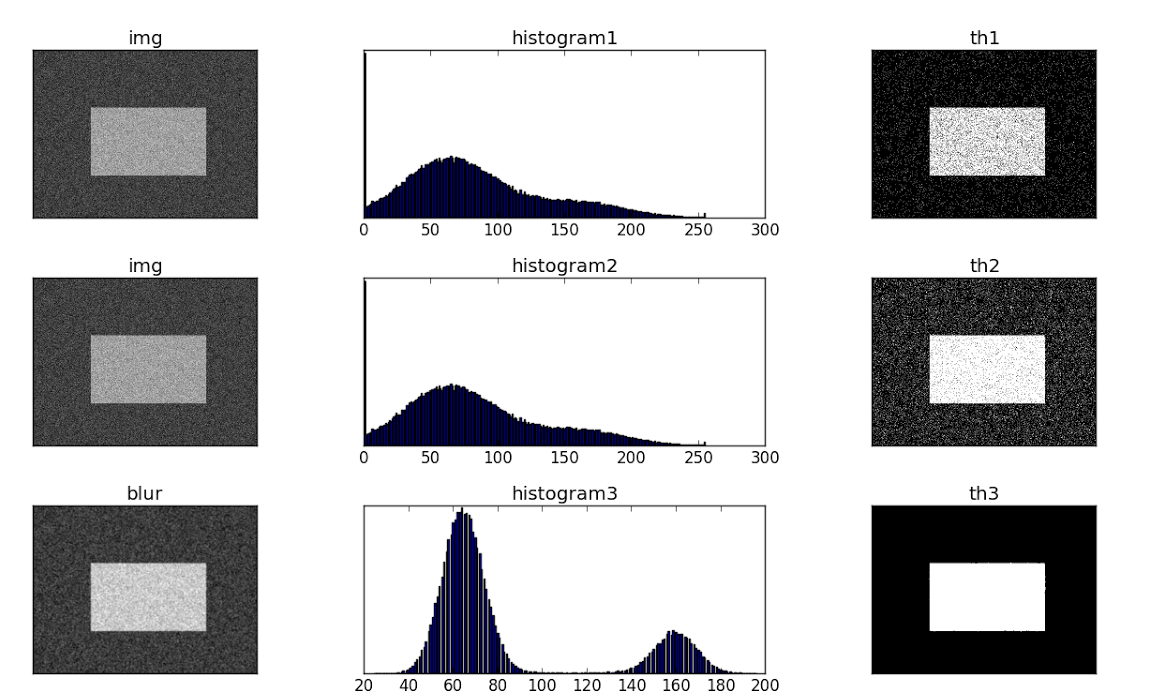
\includegraphics[width=0.8\textwidth]{otsuthres}
    \label{fig:threshold}
    \caption{Verschiedene Schwellwertverfahren im Vergleich \cite{Opencv:2013}}
\end{figure}

Reihe 1 zeigt dabei eine Schwellwertfunktion mit dem globalen Schwellwert $v=127$, in Reihe 2 wurde 
der Schwellwert mit dem Verfahren von Otsu bestimmt. In Reihe 3 wurde das Eingabebild zuerst mit einem 
Gaußfilter geglättet und weichgezeichnet, wie es auch bei der Zozosuit-Messfunktion benutzt wird. In Abbildung 
\ref{fig:thres_zozo} werden die einzelnen Bearbeitungsschritte eines Bildabschnittes mit Zozosuit veranschaulicht.


\begin{figure}[H]
    \centering
    \subfigure[Basis]{
\includegraphics[width=0.45\textwidth]{im_base}}\qquad 
    \subfigure[Graustufen]{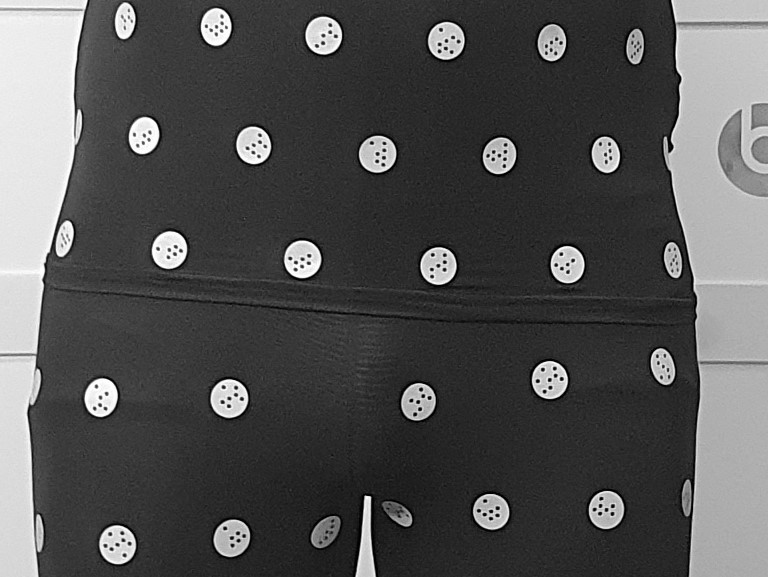
\includegraphics[width=0.45\textwidth]{im_gray}}\qquad 
    \subfigure[Gaußfilter]{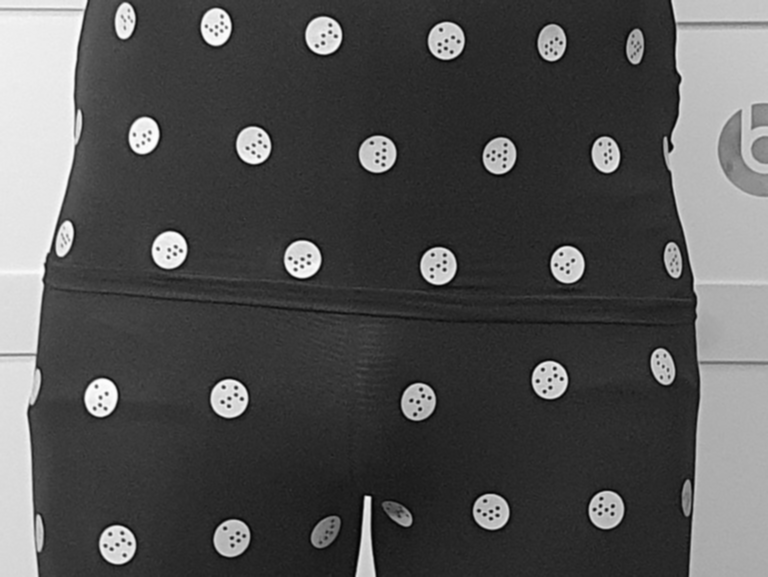
\includegraphics[width=0.45\textwidth]{im_blur}}\qquad 
    \subfigure[Schwellwert]{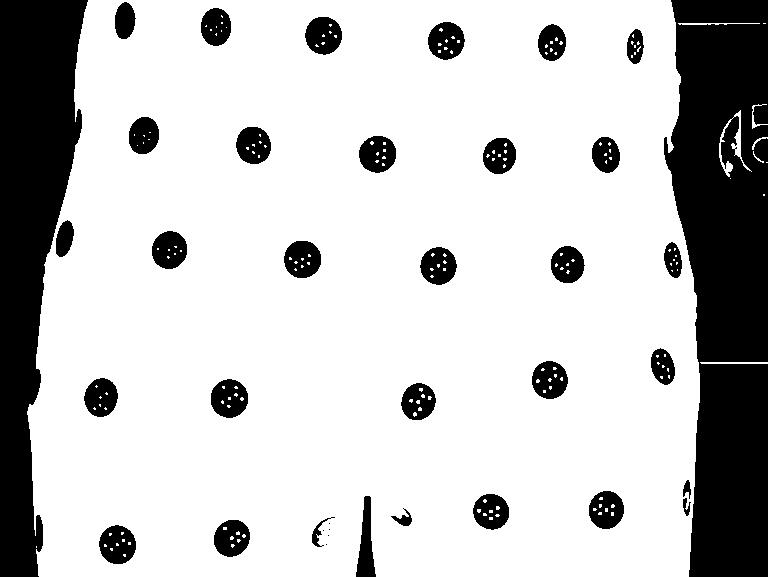
\includegraphics[width=0.45\textwidth]{im_threshold}}
    \label{fig:thres_zozo}
    \caption{Image-Pipeline bei der Aufbearbeitung des Basisbildes mit der Zozosuit-Messfunktion}
\end{figure}

Aus dem aufgearbeiteten, binären Bild werden in einem weiteren Schritt durch die OpenCV-Funktion \texttt{findContours(\dots)} die Konturen
der Messpunkte ausgelesen. Unter einer Kontur bersteht man eine Kurve, die alle Punkte entlang einer Begrenzung verbindet, welche die gleiche 
Farbe oder Itensität haben. \texttt{findContours(\dots)} gibt eine Liste von Konturen zurück, die allerdings nicht nur Messpunkte des Zozosuits
umfasst, sondern auch ungewollte Konuren. Dementsprechend müssen ungewollte Konturen gefiltert werden. Vorerst erfolgt die Entfernung
aller Konturen, die nicht in etwa zu der Größe der Messpunkte mit einem Durchmesser von 2 Centimetern passen. Konturen, die weder rund noch elliptisch sind,
können ebensfalls aussortiert werden. Da weitere Verarbeitung mit sehr flachen Ellipsen fehleranfällig ist, werden elliptische Konturen,
bei denene das Verhältnis von kürzestem Durchmesser zu längstem Durchmesser kleiner als $\frac{1}{10}$ ist, ebenfalls aussortiert. In einem
letzten Schritt erfolgt die Transformation der Elipsen zu kreisen, da diese einfacher zu verarbeiten sind. Die Transformationsmatrix wird
mit der OpenCV-Funktion \texttt{getAffineTransform(\dots)} mit drei Punkten auf berechnet, dem Mittelpunkt, dem kurzen Scheitelpunkt sowie dem langen
Scheitelpunkt. Nach der Transformation der Konturen mit der entsprechenden Transformationsmatrix ergibt sich eine Menge an Bildern der kreisförmigen Messpunkte 
des Zozosuits.

\section{Punkt auf Zozosuit}

Für die Ermittlung der einzigartigen ID eines Messpunktes ist dessen Aufbau wichtig, welcher im folgenden beschrieben wird.
Ein Messpunkt hat einen Durchmesser von 2 Centimetern, zudem existieren Messpunkte an Hals und Füßen, die nur einen Durchmesser
von einem Centimeter haben, da diese jedoch keine ID haben, spielen sie hier keine Rolle. In jedem der circa 300 Messpunkten befindet
sich eine Anordnung von 4 bis 10 kleinen Pünktchen mit einem Durchmesser von 2 Millimeter, welche eine einzigartige ID wie folgt widerspiegeln, sowie ein
Pünktchen im Mittelpunkt.
\begin{figure}[t]
    \centering
    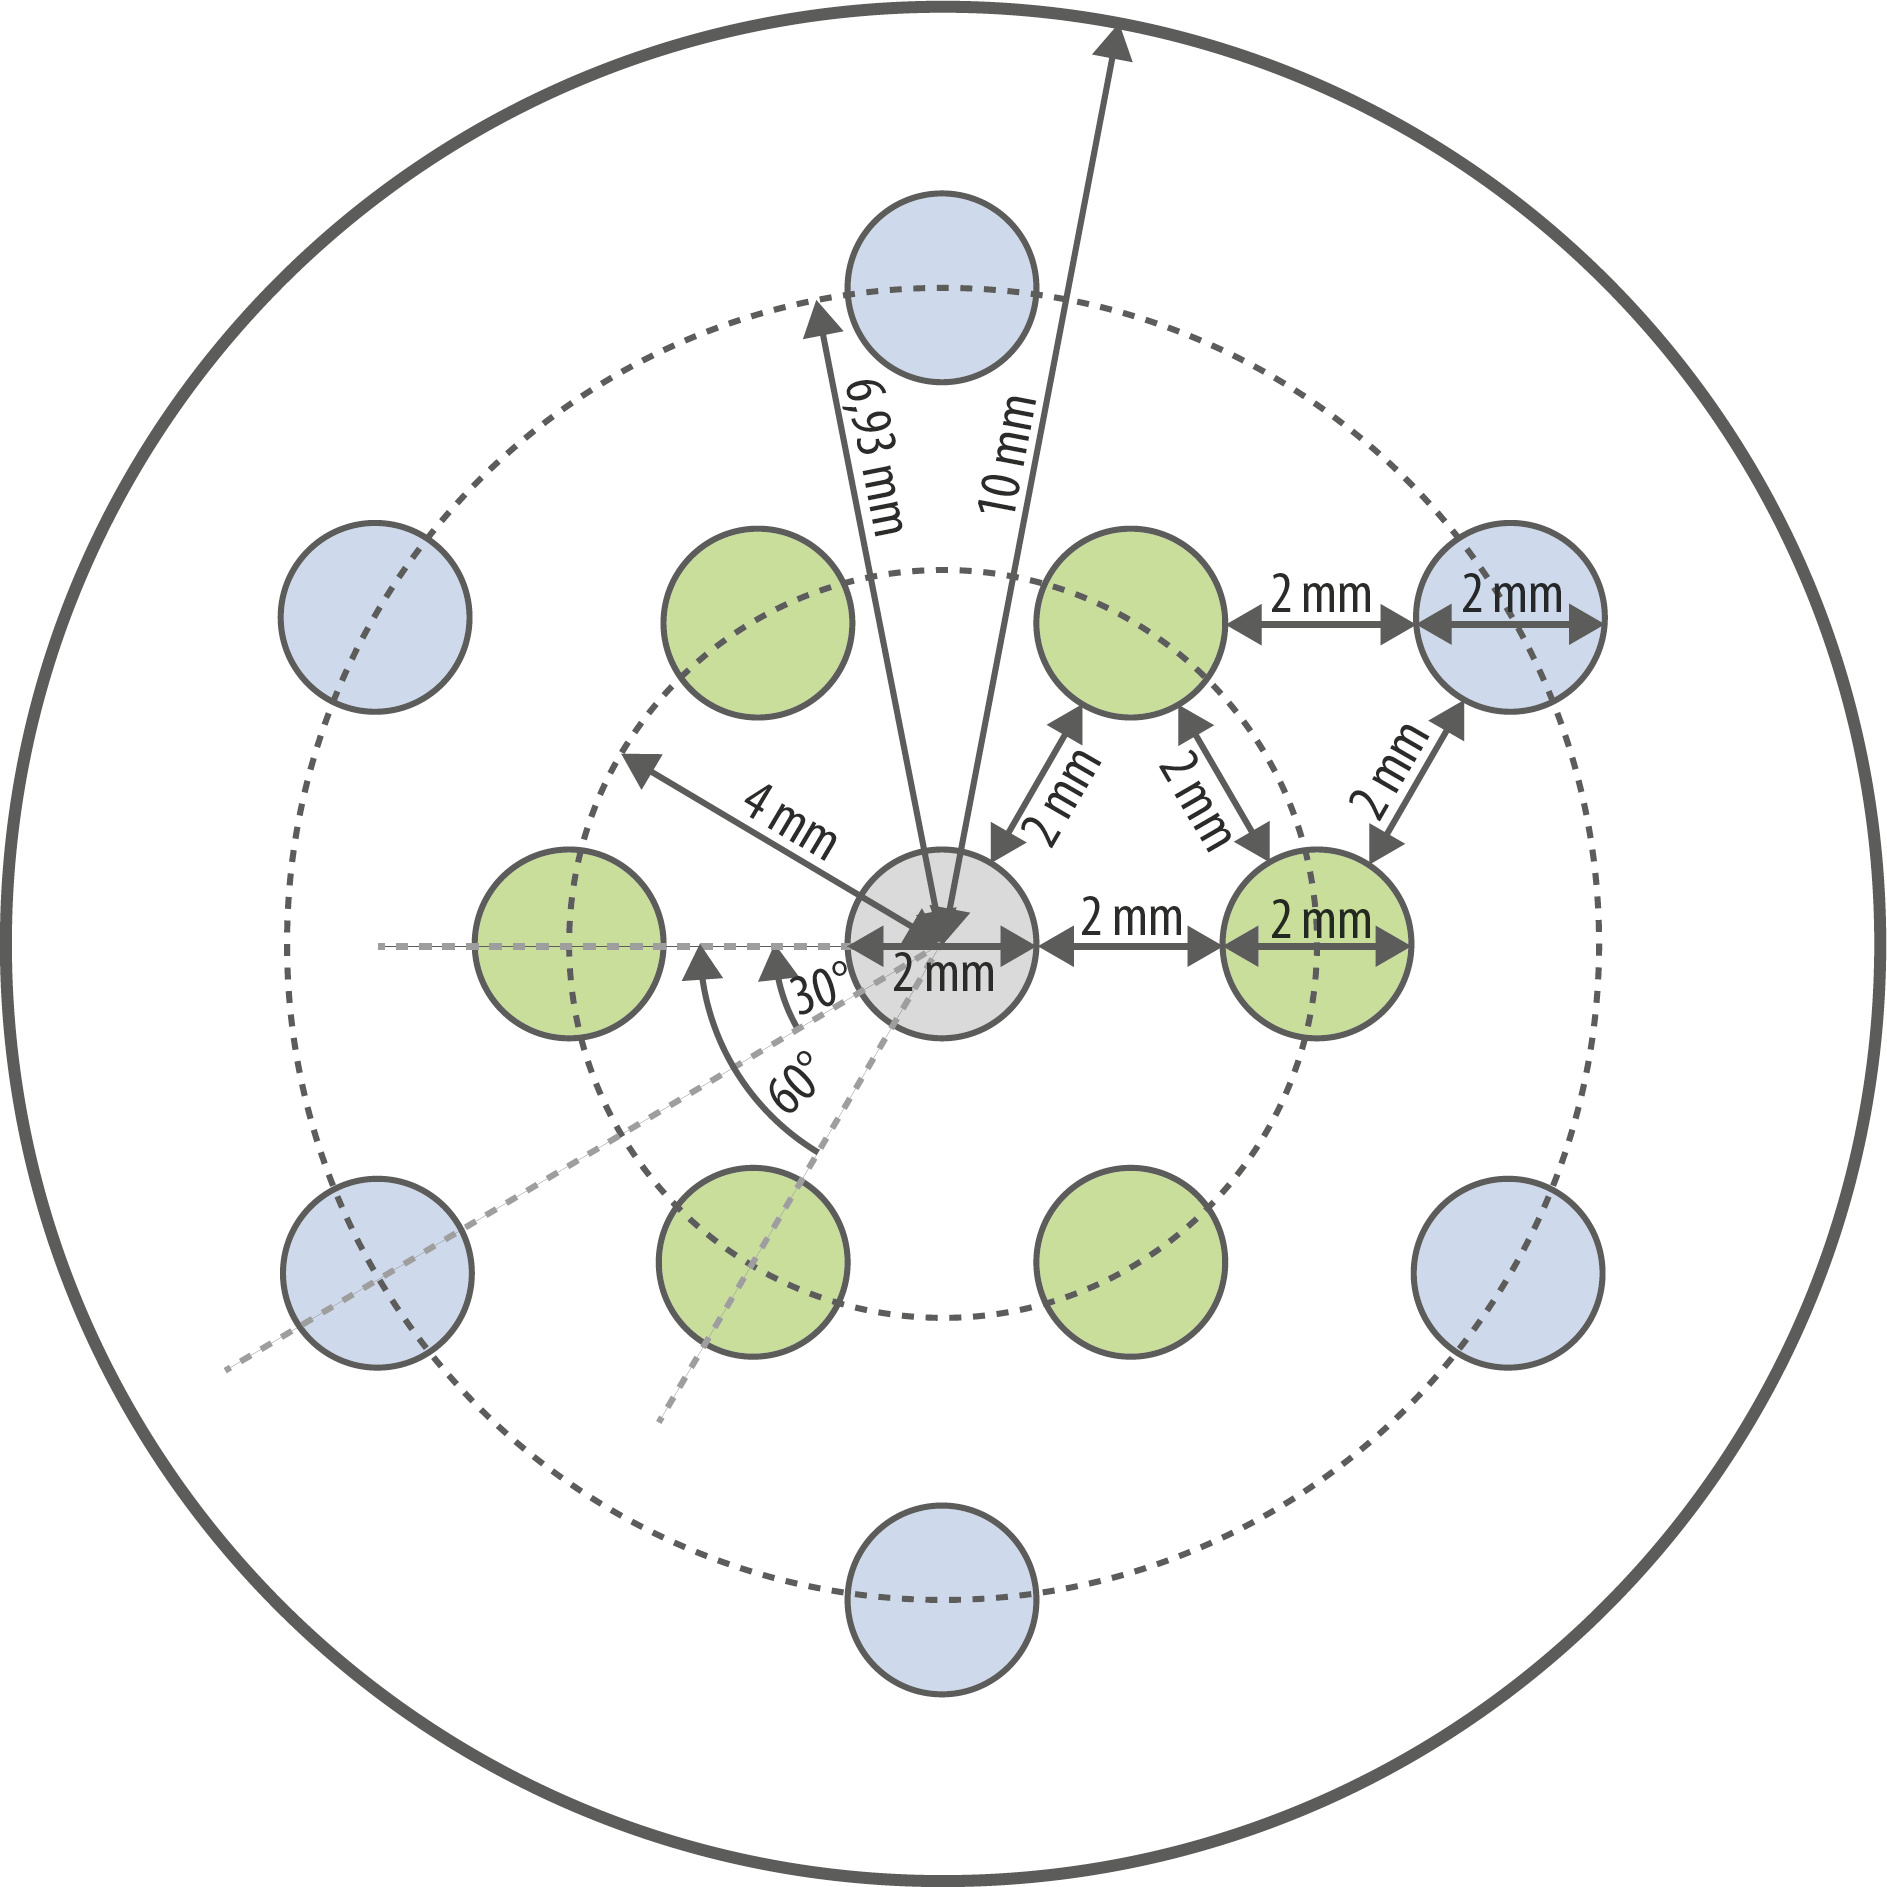
\includegraphics[width=0.9\textwidth]{Zozopunkt}
    \label{fig:zozopunnkt}
    \caption{Aufbau eines Messpunktes des Zozosuits \cite{Pina:2018}}
\end{figure}
In einem Messpunkt befinden sich je 6 mögliche Positionen für Pünktchen auf einem Kreis mit dem Radius von 4 Millimeter und einem Winkel von 60° zum 
Nachbarn. Weitere 6 mögliche Positionen befinden sich auf einem Kreis mit dem Radius von etwa 6.93 Millimetern, ebenfalls mit einem WInkel von 60° zudem
Nachbarn, allerdings um 30° zu jenen Positionen im inneren Kreis (vgl. Abb. \ref{fig:zozopunnkt}).

So ergeben sich insgesamt 12 mögliche Positionen für Pünktchen, welche je ein Bit kodieren. Existiert ein Pünktchen auf einer Position,
ist der Bitwert 1, ansonsten. Dies ergibt eine $2^12=4096$ möglichen Punkteanordnungen. Die Pünktchen des äußeren Kreises kodieren im
Uhrzeigsinn gehend, beginnend beim Pünktchen im Norden, die ersten 6 Bits. D Pünktchen im inneren Kreis stellen im Uhrzeigersinn gehen, angefangen
beim Pünktchen um 30° im Uhrzeigsinn verschoben zum Norden, die zweiten 6 Bit dar. Allerdings müssen sich bei jedem Messpunkt 
sowohl auf dem inneren Kreis als auch dem 
äußeren Kreis mindesten 2 und maximal 5 Pünktchen befinden. Da die Messpunkte in der Wirklichkeit (um 60°,120°,180°,240°,300°) verdreht sein können, werden zudem nur jene der
6 möglichen Punkteanordnung gezählt, deren 12 Bit die höchste Zahl kodieren. Diese beiden Einschränkungen ergeben eine Anzahl von 608 einzigartigen
IDs für die 2 Centimeter großen Messpunkte. \cite{Pina:2018}

\section{Erkennung der ID}

Für die Erkennung der ID eines Messpunktes auf dem Zozosuit muss dieser zuerst in eine Position gedreht werden, sodass die Positionen
der Pünktchen mit jene in Abbildung \ref{fig:zozopunnkt} übereinstimmen. Hierbei wird eine Maske mit den 12 möglichen Punktepositionen
erzeugt über dem Messpunkt erzeugt und 60 Mal um 1° verschoben. Ist diese Maske so gedreht wie die tatsächlich vorhandenen Pünktchen 
im Messpunkt, haben die maskierten Pixel eine kleinere durchschnittliche Helligkeit als alle Masken mit abweichendem Winkel. 
Mit dem nun richtig gedrehten Messpunkt kann die ID ermittelt werden. Hier werden 12 Masken, die je eine der 12 Punkteposition freistellen,
über den Messpunkt gelegt. Liegt der durchschnittliche Farbwert der so freigestellten Punkteposition über dem Mittelwert von 127, wird davon ausgeganen,
dass sich auf dem Messpunkt an dieser Stelle ein Pünktchen befindet, was als binäre 1 interpretiert wird. Liegt der durchschnittliche Farbwert
unter dem Mittelwert von 127, befindet sich an dieser Stelle kein Pünktchen und der binäre Wert wird auf 0 gesetzt. Dieser Vorgang wird 12 Mal wiederholt,
sodass jeder Punktepositionen ein binärer Wert zugewiesen wird. \cite{Pina:2018}

Zusammengesetzt ergibt sich dadurch eine 12-Bit ID. Da jedoch 5 weitere mögliche Ausrichtungen des Punktes möglich sind, und die IDs 
konsistent sein sollen, wird wie im letzten Kapitel beschrieben immer nur die höchst mögliche ID der 6 verschiedenen Drehungen der Punkteanordnung
verwendet. Hierbei wird 6 Mal je auf die ersten und letzten 6 Bit ein Bitshift nach links durchgeführt, das 1. Bit an die 7. Position kopiert und
und das 1. Bit gelöscht. Der höchste enstehende binäre Werte ist die ID des Punktes. \cite{Pina:2018}

\newcommand{\irow}[1]{% inline row vector
\big[ \  #1 \ \big]%
}

\chapter{Punkteverarbeitung}

3D-Objekte werden oft durch Scheitelpunkte und Dreiecke dargestellt, welche deren dreidimensionale Form widerspiegelt.
Dabei gilt, je detaillierter ein Objekt ist, desto mehr Scheitelpunkte werden benötigt. Bei einem Objekt wie dem
Menschen mit weitgehend vordefinierter Form kann die Darstellung jedoch auf einige wenige Größen wie Höhe,
Dicke, Brustumfang, Bauchgröße und Pose reduziert werden. Diese Darstellung ist oft kleiner und aussagekräftiger.
\cite{Ha2018} Die Idee ist die Entwicklung einer Funktionalität, welche die Rückgabewerte der
Messfunktion als Eingangsparameter für die Erstellung eines Modells mit STAR nutzbar macht.

\section{STAR}

Eine dieser Darstellungen ist der Sparse Trained Articulated Human Body Regressor (STAR). 
STAR ist ein statistisches Modell, das den menschlichen Körper mit zwei Parametern, dem Shape-Parameter $\boldsymbol{\beta}$
für die Form und dem Pose-Parameter $\boldsymbol{\Theta}$ für die Pose, beschreibt.

\subsection{Shape}

Einer der beiden Parameter für die Generierung des Modells eines menschlichen Kröpers mit STAR ist der sogenannte Shape-Parameter.
Dieser umfasst 10 bis 300 Skalare \linebreak ${\boldsymbol{\beta}= \irow{\beta _0 \ ,\ \ldots \ , \ \beta_{|\beta|}}}$, welche die
Form des menschlichen Körpers widerspiegeln. Jedes Skalar erwirkt bei der Modellgenerierung eine
Veränderung eines bestimmten Merkmals. Das Skalar $\beta _0$ ist dabei beispielsweise ausschlaggebend
für die Größe des Modells, $\beta _1$ wirkt auf das Verhältnis von Körpergröße und Gewicht, ähnlich wie
der Body Mass Index. Der Wert für $\beta _2$ bestimmt die Höhe des Torsos und Schulterbreite, jener für
$\beta _3$ die Brustbreite sowie Nackenhöhe.
\begin{figure}[H]
  \centering 
   \subfigure[negativ]{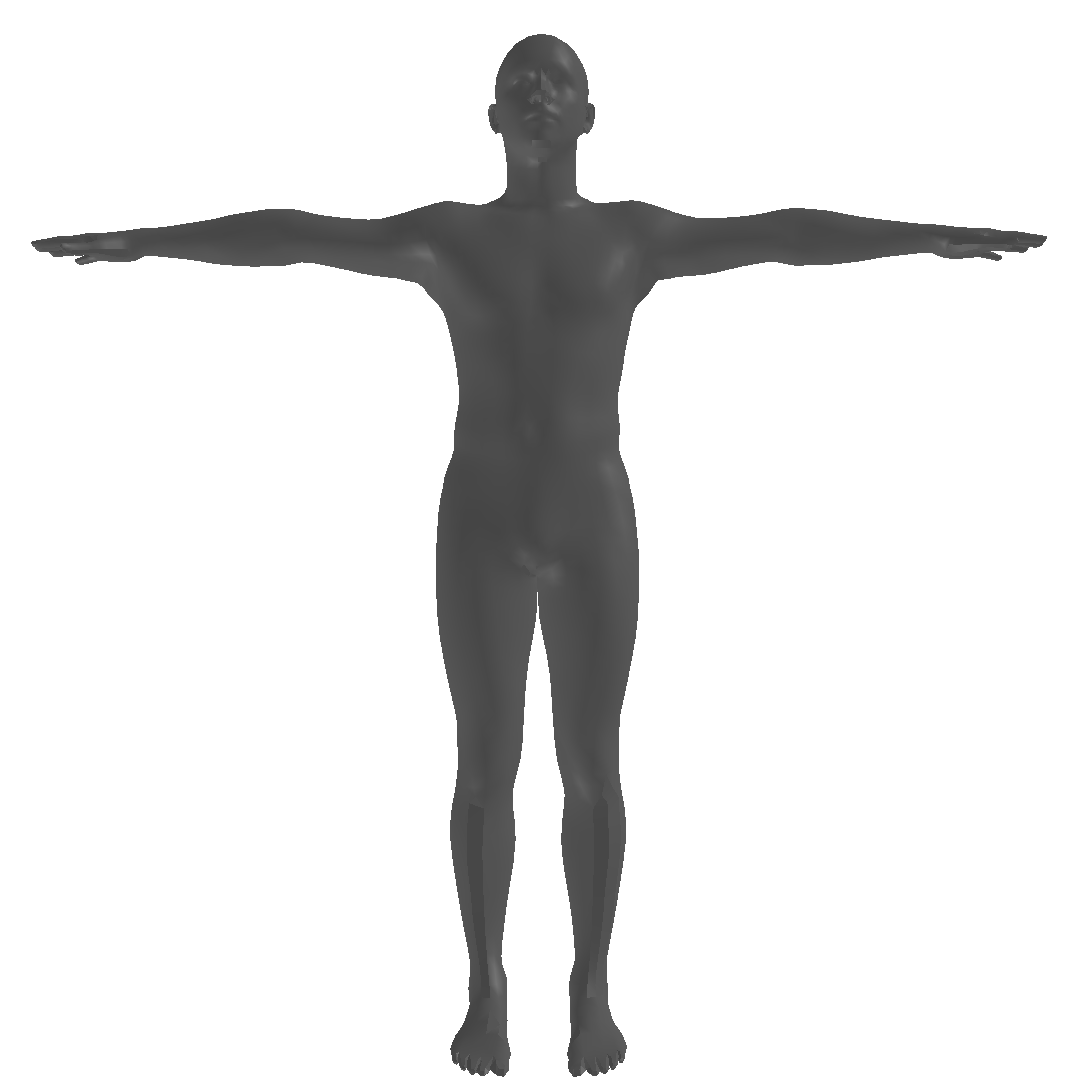
\includegraphics[width=0.4\textwidth]{shape_slim}}\qquad 
   \subfigure[positiv]{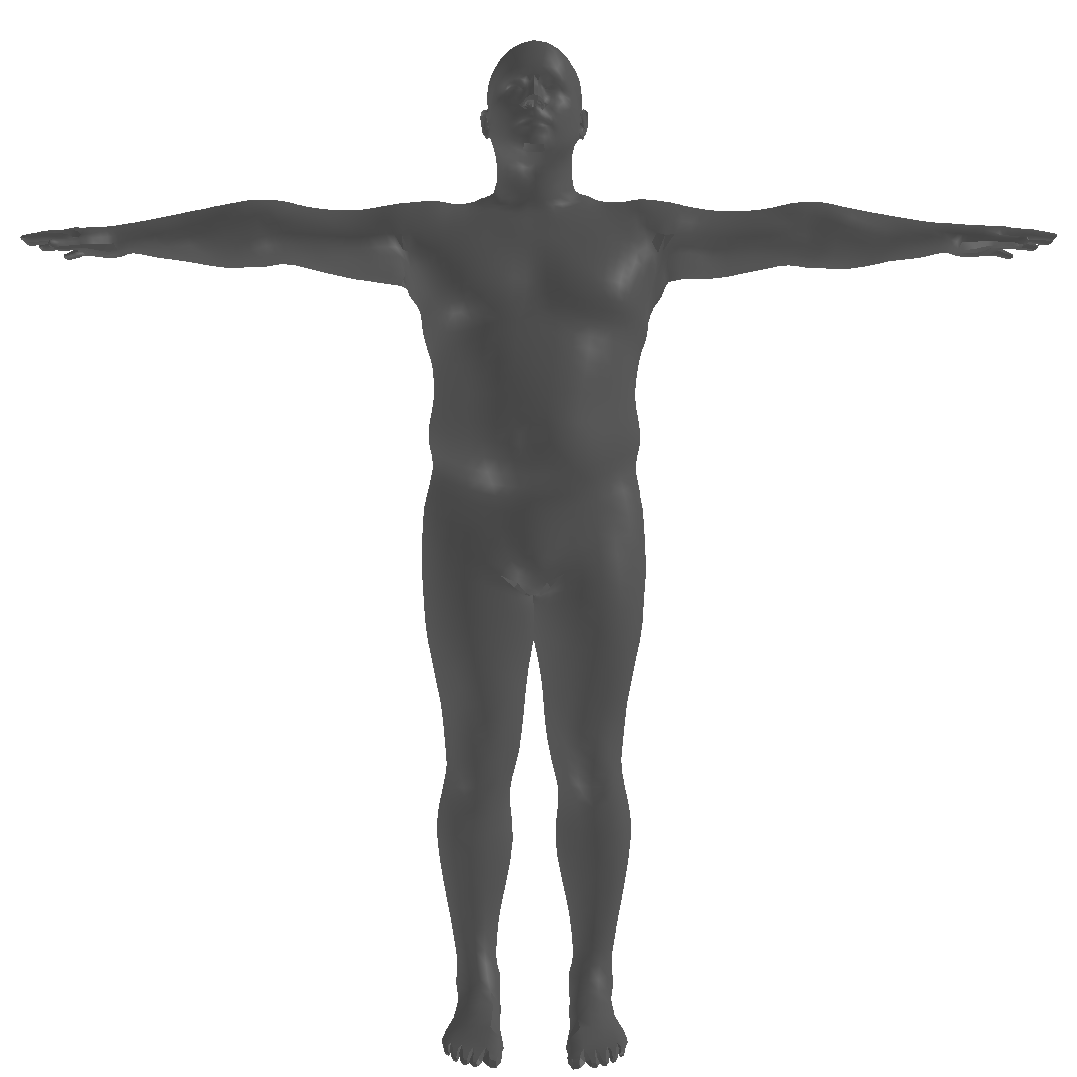
\includegraphics[width=0.4\textwidth]{shape_big}}\qquad 
   \subfigure[default (=0)]{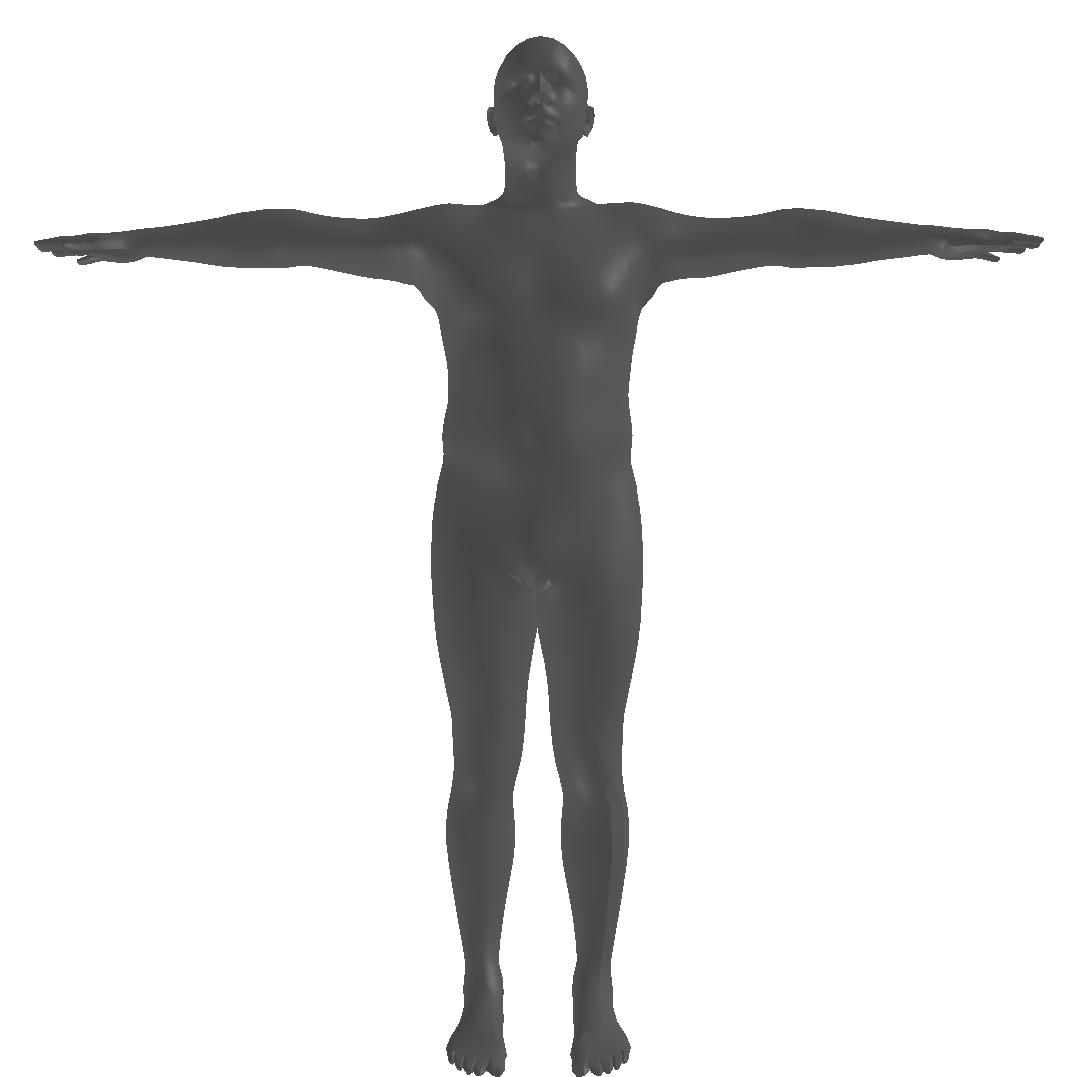
\includegraphics[width=0.4\textwidth]{shape_normal}}
  \caption{Gerenderte Modelle mit verschiedenen Shape-Parametern} 
  \label{fig:betas}
\end{figure}

Ein negativer Wert für ein Skalar reduziert dabei das
entsprechende Merkmal, ein positiver Wert verstärkt dieses (vgl. Abb. \ref{fig:betas}). Je höher dabei die Anzahl an Skalaren,
desto genauer lässt sich das Modell an einen bestimmten Körperbau anpassen, im Gegenzug
erhöht sich aber der Rechenaufwand.

\subsection{Pose}

Der zweite Eingabeparameter für STAR ist der Pose-Parameter, welcher die zu generierende Pose
mit 24 Vektoren ${\boldsymbol{\Theta}=\irow{\vec{\Theta} _0 \ ,\ \ldots \ , \ \vec{\Theta} _{23}}}$, die
je 3 Skalare ${ \vec{\Theta} _n=\irow{x_n \ ,\ y_n \ ,\ z_n}}$ umfassen, beschreibt. Die Vektoren
werden als Rotation in Axis-Angle-Darstellung von Gelenken des menschlichen Körpers relativ
zum Vorgängergelenk interpretiert, welche zusammengesetzt einen sogenannten Kinematischen
Baum mit den wichtigsten Gelenkpunkten ergeben (vgl. Abb. \ref{fig:axisangle}, (b)). Die Axis-Angle-Darstellung
beschreibt die Drehung eines dreidimensionalen Objekts um den Winkel $\Theta$ um eine Rotationsachse
mit dem Einheitsvektor $\vec{e}$. Diese beiden Variablen können mit $\Theta * \vec{e}$ als Vektor mit drei Parametern und dem Betrag $\boldsymbol{\Theta}$
zusammengefasst werden. (vgl. Abb. \ref{fig:axisangle}, (a)).

\begin{figure}[H]
  \centering 
   \subfigure[]{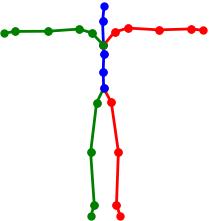
\includegraphics[width=0.45\textwidth]{joints}}\qquad
   \subfigure[]{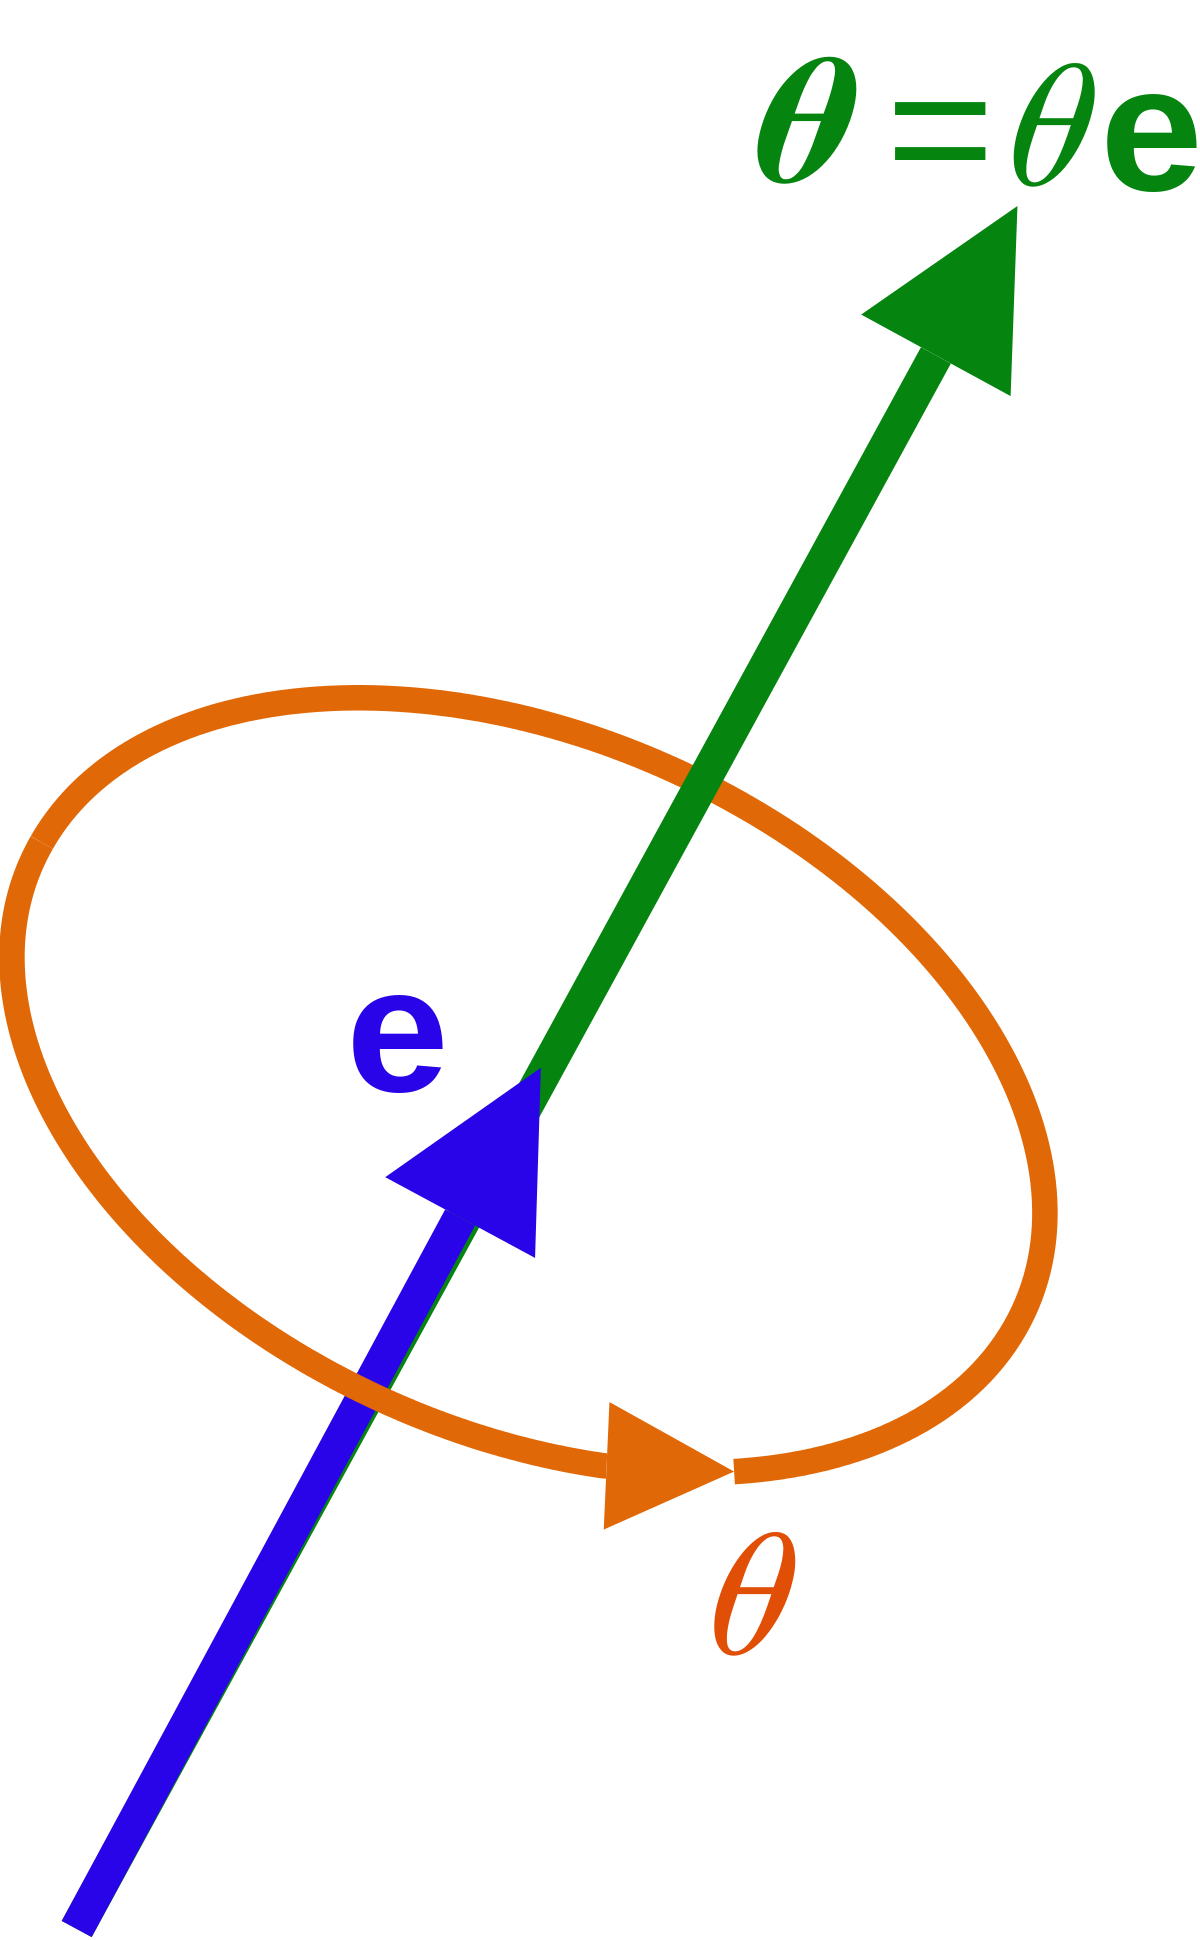
\includegraphics[width=0.3\textwidth]{Angle_axis_vector}}
  \caption{Gelenke des STAR-Modells (a) und Axis-Angle-Darstellung einer Rotation \cite{wiki:Axis–angle_representation} (b)} 
  \label{fig:axisangle}
\end{figure}

\newpage
Dabei gilt, je kleiner der Wert eines Skalars gegenüber den anderen beiden Skalaren, desto geringer
ist die Drehung entlang der entsprechenden X-Achse, Y-Achse oder Z-Achse. Ein Drehung um $\frac{\pi}{2}$ um die
X-Achse und $\frac{\pi}{2}$ um die Y-Achse entspräche $\irow{0.89*\frac{\pi}{2} \ ,\ 0.45* \frac{\pi}{2} \ ,\ 0}$ in 
Axis-Angle-Darstellung. Durch verschiedene Gewichtungen der 24 Vektoren kann so jede erdenkliche Pose
dargestellt werden (vgl. Abb. \ref{fig:poses}, (b)). Sind die Elemente eines Vektors $\vec{\Theta _n} = \irow{0 \ , \ 0 \ ,\ 0}$, befindet sich das Gelenk in Ruheposition.
Abbildung \ref{fig:poses} (a) zeigt das Modell, bei dem sich alle Gelenke in Ruhepose befinden.

\begin{figure}[H]
  \centering 
   \subfigure[Ruhepose]{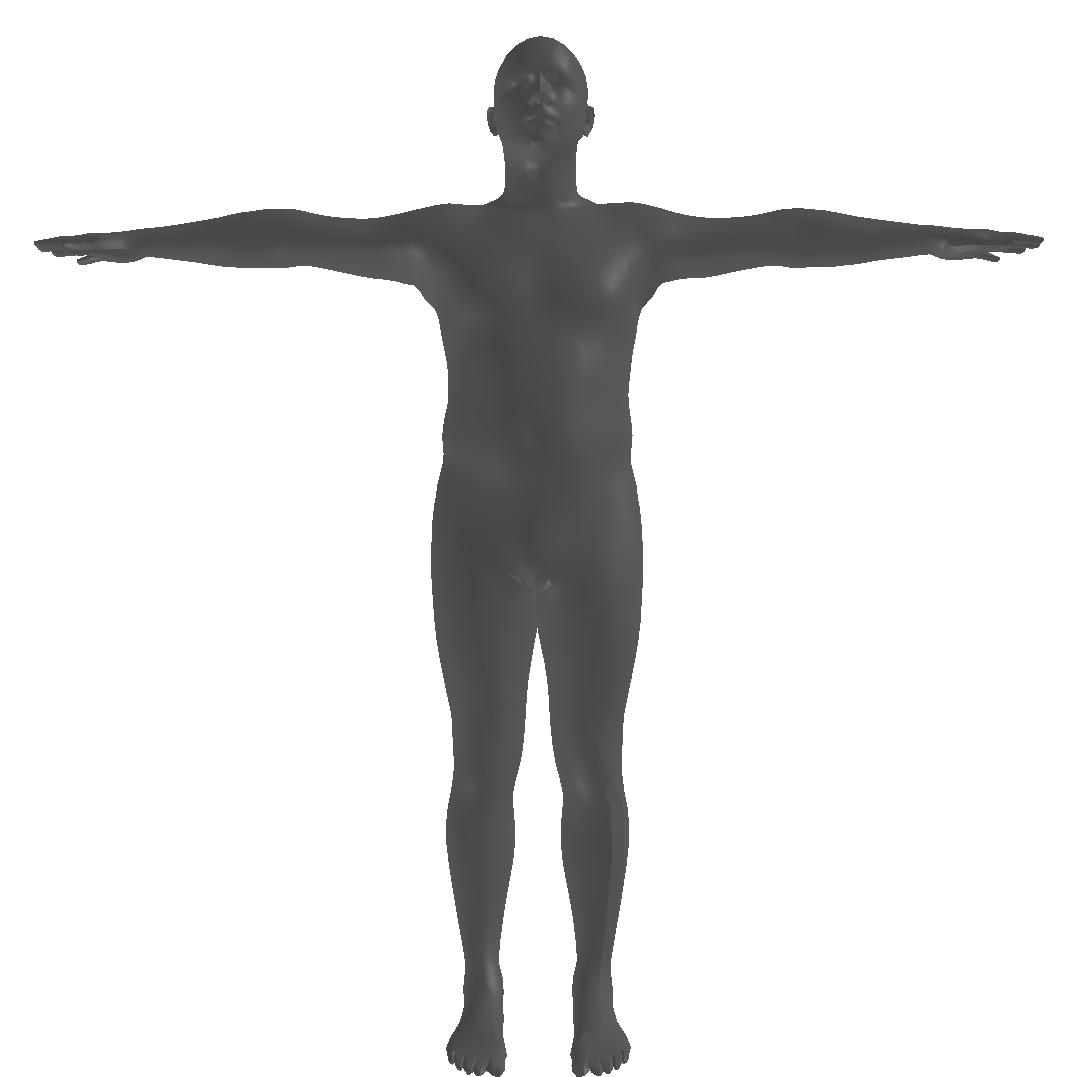
\includegraphics[width=0.4\textwidth]{pose0}}\qquad 
   \subfigure[Zufällige Pose]{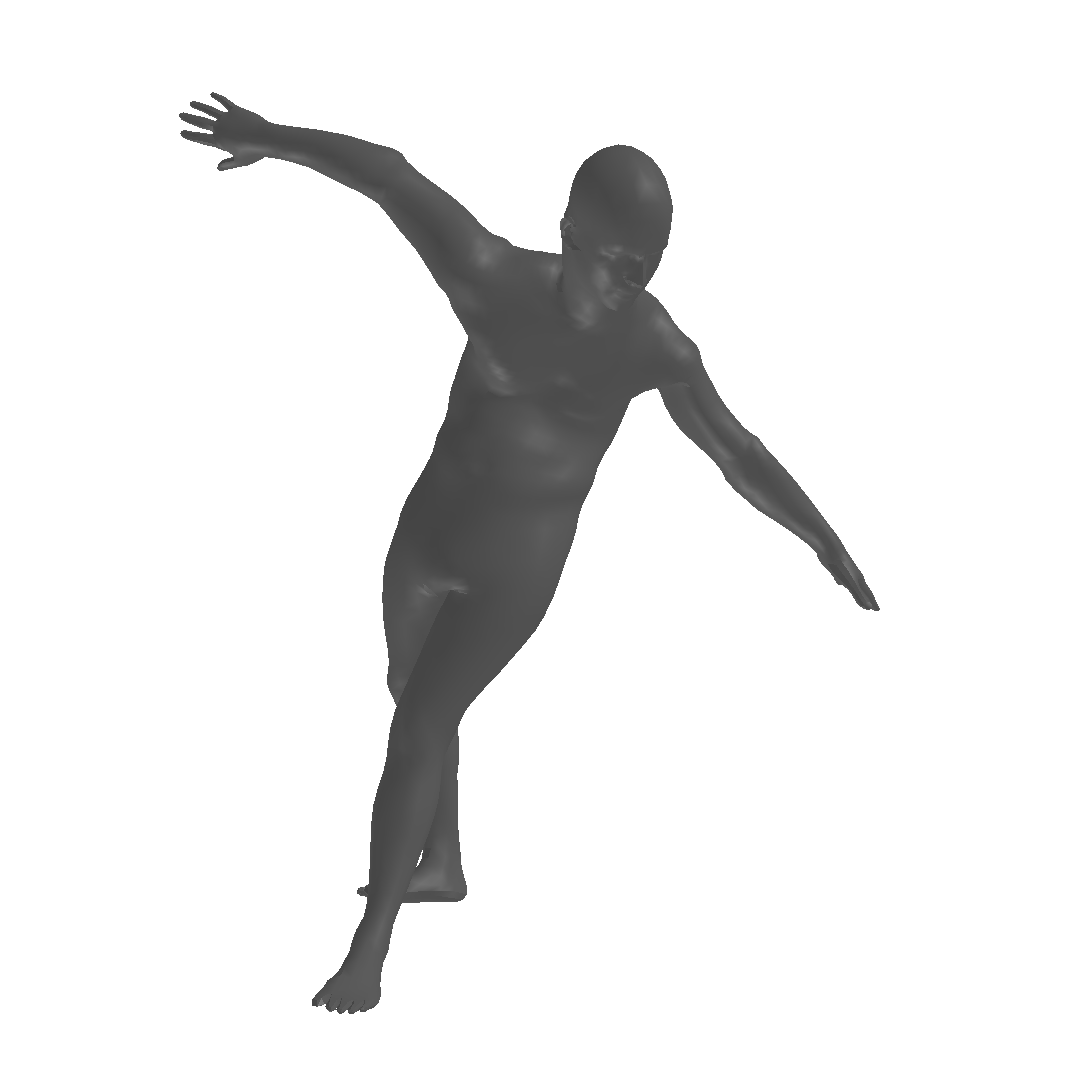
\includegraphics[width=0.4\textwidth]{pose1}}
  \caption{Gerenderte Modelle mit verschiedenen Pose-Parametern} 
  \label{fig:poses}
\end{figure}

\subsection{Funktionsweise}

Die Pipeline der Synthese des menschlichen Körpers mit Star erfolgt in drei Schritten. In einem ersten Schritt wird ein
Template-Modell $\overline{T}$ in Ruhepose und ohne Form-Korrekturen erstellt und Scheitelpunktversätze zum Modell T mit der Funktion
$B_s(\beta;S)$ berechnet. Der Parameter $S$ beschreibt dabei vordefinierte grundlegende Komponenten, welche den Bereich der
menschlichen Formvariabilität erfassen. Addiert ergeben Modell $\overline{T}$ und Scheitelpunktversätze
$\vec{V}_{shaped}$, ein Modell in Ruhepose,
das die mit den Shape-Koeffizienten definierten physikalischen Attribute und die Identität widerspiegelt.

\begin{equation}\label{eq:Star_Vshaped}
  \vec{V}_{shaped}=\overline{T}+B_s(\beta;S)
\end{equation}

Der menschliche Körper verformt sich in unterschiedlichen Posen anders, was für ein realistisches Ergebnis in Betracht
gezogen werden muss. Diese Verformung ist zudem abhängig von der Form des Körpers. Der zweite Schritt dient dementsprechend der
Berechnung der durch die Pose $\Theta$ verursachten Verformungen in Korelation mit den Shape-Koeffizienten $\beta$ durch die Funktion
$B_p(\vec{q},\beta _1) $. Der Parameter $\vec{q}$ stellt dabei den kinematischen Baum als Quaternion mit je vier
Parametern pro Skelettpunkt dar. $\beta _1$, also der
zweite Koeffizient des Shape-Parameters, ist repräsentativ für die allgemeine Form des Körpers und stimmt in vielen
Punkten mit dem Body Mass Index (BMI) überein. Da $\beta _1$ den mit Abstand größten Einfluss auf die Verformungen durch
spezielle Posen hat, können die restlichen Shape-Koeffizienten vernachlässigt werden. Das Endresultat $\vec{V}_{posed}$, gegeben
durch

\begin{equation}\label{eq:Star_Vposed}
  \vec{V}_{posed}=\overline{T}+B_s(\beta;S)+B_p(\vec{q},\beta _1)
\end{equation}

stellt nun ein Modell in Ruhepose dar, das sowohl Verformungen durch den Shape-Parameter als auch durch den
Pose-Parameter umfasst. Da das Modell $\vec{V}_{posed}$ posenspezifische Verformungen umfasst, aber trotzdem in Ruhepose dargestellt
wird, kann ein leicht unförmiger Eindruck entstehen. 

Im dritten und letzten Schritt, dem sogenannten Skinning, wird das Mesh mit einer standard skinning Funktion $\mathcal{W}$  um die Joints von $\vec{V}_{shaped}$ transformiert sowie durch ein erlerntes Set aus blend weight parametern geglättet. Das Modell ist schlussendlich gegeben durch

\begin{equation}\label{eq:Star_Model}
  M(\vec{\beta},\vec{\Theta})=W(T_p(\vec{\beta},\vec{\Theta}), J(\vec{\beta},\vec{\Theta}, \mathcal{W}))
\end{equation}

Die Funktion $J$ regressiert dabei die Joints zwischen den Skelettpunkten aus $\vec{V}_{shaped}$. Das so synthetisierte Modell des
menschlichen Körpers ist realistisch und weicht bei richtiger Messung und Parametrierung von Shape und Pose um nur wenige
Millimeter ab. Ziel des folgenden Kapitels ist die Entwicklung einer Funktionalität, welche die Rückgabewerte der
Messfunktion als Eingangsparameter für die Erstellung eines Modells mit STAR nutzbar macht.

\section{Verarbeiung}

Um mittels Star ein realistisches Modell des menschlichen Körpers zu generieren, müssen die Rückgabewerte der
Measure-Funktion zu Shape-Parameter $v{\beta}$ und Pose-Parameter $\boldsymbol{\Theta}$ konvertiert werden. Im folgenden wird die Idee der Konvertierung, die Umsetzung sowie aufgetretene
Probleme dargestellt.

\subsection{Idee}

In allen großen Messpunkten des Zozosuits befindet sich eine einzigartige Punkteanordnung, wodurch jedem gescannten
Messpunkt eine ID und somit eine entsprechende Position auf dem Zozosuit zugewiesen werden kann. Diese ID wird von der Measure-Funktion, neben den genauen Koordinaten und einer geschätzten Entfernung des
Punktes, erfasst. Dadurch lässt sich eine dreidimensionale Punktewolke erzeugen und die genauen Koordinaten eines
Messpunktes auf dem Zozosuit mit der ID ermitteln.

Die Pose kann so durch Zuweisung von passenden Punkten des Zozosuits zu den Gelenkpunkten des
Pose-Parameters rekonstruiert werden. Hierfür ist es erforderlich, die Rotation In
Axis-Angle-Darstellung zu berechnen, welche den Vektor zwischen zwei Gelenkpunkten des kinematischen Baums der Ruhepose zu dem 
Vektor zwischen den zwei entsprechenden Punkten auf dem Zozosuit rotiert.

Die Ermittlung des Shape-Parameters erweist sich als komplexer. Die bis zu 300 verschiedenen Skalare, welche auch in
gegenseitiger Wechselwirkung stehen, zu erschließen, ist mit den Daten, die die Messfunktion des Zozosuit liefert,
unmöglich. Allerdings könnte man nur einige wenige der Skalare betrachten, welche einen großen Einfluss auf die
allgemeine Form haben, wie die Skalare $\beta _0$ und $\beta _1$, welche die Größe sowie den Body Mass Index des Modells beschreiben. Diese können 
durch Messung von Entfernungen verschiedener bestimmter Punkte grob bestimmt werden. Dies soll aber im Rahmen
der Arbeit dieser Arbeit nicht näher betrachtet werden.

\subsection{Umsetzung}
Für die Ermittlung der Pose aus den Daten der Zozosuit-Messfunktion erfolgt in 
einem ersten Schritt die Zuweisung der IDs von Messpukten zu den Gelenkpunkten des Pose-Parameters.
 Dies wird einmalig durch einen Vergleich von Gelenkpunkten des Kinematischen Baums und 
Messpunkten auf dem Zozosuit ermittelt.

\begin{figure}[H]
  \centering 
   \subfigure[Erfasste Punkte]{\includegraphics[width=0.3\textwidth]{point_positions}}\qquad 
   \subfigure[Numerierte Joints des STAR-Modells \cite{STAR:2020}]{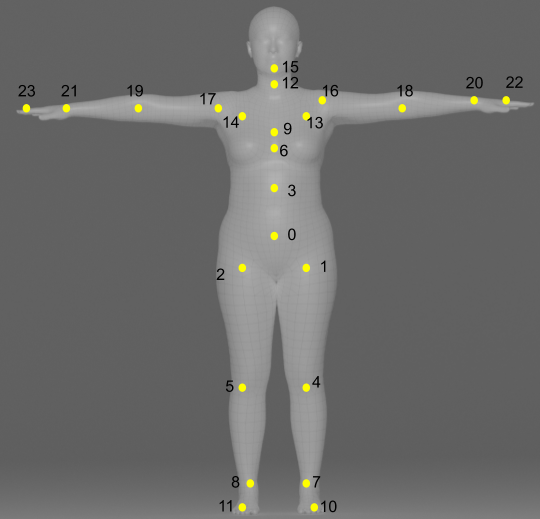
\includegraphics[width=0.6\textwidth]{star_kinematic_tree}}
  \caption{Vergleich von Joints des Star-Modells und Punkten des Zozosuits mit IDs in Gelb} 
  \label{fig:pointpos}
\end{figure}

Die Koordinaten der Messpunkte, deren ID mit einem Gelenkpunkt verknüpft ist, werden aus dem Rückgabewert
\texttt{raw\_data} als dreidimensionale Punktewolke ausgelesen. Da der Pose-Parameter Rotationen von Gelenk zu 
übergeordnetem Gelenk gemäß des kinematischen Baums benötigt, ist eine Konvertierung der Punktewolke zu Rotation in 
Axis-Angle-Darstellung erforderlich. Die Rotation eines Gelenks wird dabei relativ zur Rotation des Gelenks in Ruhepose berechnet.
In anderen Worten muss die Rotation des Vektors \texttt{v\_src} von übergeordnetem Gelenkpunkt zu Gelenkpunkt
der Ruhepose zu Vektor \texttt{v\_dst} von übergeordnetem Gelenkpunkt zu Gelenkpunkt der Messpose berechnet werden. Hierfür dient die
Funktion \texttt{axis\_angle(v\_src,v\_dst)}, welche die Rotation von \texttt{v\_src} zu \texttt{v\_dst} in Axis-Angle-Darstellung zurückgibt.

In der Funktion \texttt{axis\_angle(\dots)} werden in einem ersten Schritt werden beide Vektoren genormt, da lediglich
die Richtung der Vektoren bei der Berechnung der Rotationsmatrix eine Rolle spielen. Die Rotationsachse
ist definiert durch das Kreuzprodukt von Ursprungsvektor und Zielvektor, der Winkel der Drehung durch den
Arkustangens des Skalarprodukts der beiden Vektoren. Demnach lässt sich die Drehung eines Vektors 
$\vec{v}_{src}$ zu einem Vektor $\vec{v}_{dst}$ in Axis-Angle-Darstellung mit

\begin{equation}\label{eq:axis_angle}
  \boldsymbol{\Theta} = \Theta * \vec{e} = \arctan(\vec{v}_{src} \cdot \vec{v}_{dst}) * \lVert \vec{v}_{src} \times \vec{v}_{dst} \rVert
\end{equation}

berechnen. Nachdem dies für alle Gelenke berechnet wird, lässt sich mit Hilfe von Star ein Modell generieren, welches
die Pose der Person auf dem Bild widerspiegelt. Allerdings treten dabei einige Probleme auf, die das Ergebnis
stark verzerren können, welche im folgenden vorgestellt werden.

\subsection{Probleme}
Bei der Synthese der Pose aus den Messpunkten des Zozosuit treten eine Reihe von Problemen auf.

\subsubsection*{Fehlende Messpunkte an Gelenken}
Eine Problem ist, dass nicht für jedes Gelenk ein Messpunkt auf dem Zozosuit existiert. Einige
Gelenke müssen deshalb komplett ausgelassen werden, wie beispielsweise jene an Kopf, Füßen und Händen, da kein Messpunkt in der
Nähe existiert. Diese sind für die gesamte Pose aber nicht ausschlaggebend. Deshalb wird für diese die Ruhepose des Gelenkes
$\boldsymbol{\Theta}=\irow{0 \ , \ 0 \ ,\ 0}$ verwendet. Bei anderen Gelenken, vor allem in der Schulterregion liegen die Messpunkte
lediglich in der Nähe des Gelenks (vgl. Abb. \ref{fig:schulter}).

\begin{figure}[H]
  \centering 
   \subfigure[Erfasste Punkte in der Schulterregion]{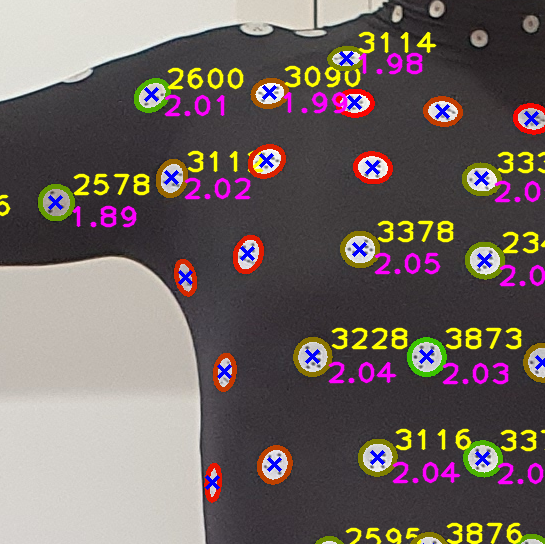
\includegraphics[width=0.475\textwidth]{point_positions_schulter}}\qquad 
   \subfigure[Gelenke in der Schulterregion \cite{STAR:2020}]{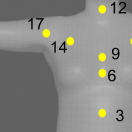
\includegraphics[width=0.475\textwidth]{star_kinematic_tree_schulter}}
  \caption{Vergleich von Joints des Star-Modells und Punkten des Zozosuits mit IDs in gelb} 
  \label{fig:schulter}
\end{figure}

Dadurch wird die Pose verzerrt, Beispiele hierfür sind leicht falsch abstehende Arme oder gespreizte Beine. Zwar können 
einige Gelenke durch Zusammenspiel von mehreren Messpunkten berechnet werden, allerdings 
wird der Effekt durch das nachfolgend beschriebene Problem verstärkt.

\subsubsection*{Lückenhafte Punkterkennung}
Bei der Erkennung der Messpunkte mit der Zozosuit-Messfunktion werden häufig Punkte gar nicht oder ohne
ID erkannt. Die dadurch entstehende lückenhafte dreidimensionale Punktewolke der Messpose hat zur Folge, dass
nicht alle Pose-Parameter berechenbar sind. Jeder fehlende Messpunkt, mit Ausnahme der Start- und Endpunkte, 
verursacht zwei fehlende Pose-Parameter, die zur Ruhepose des Gelenks gesetzt werden müssen. Dadurch kommt es teils
zu einer Pose des Modells, die einigen essentiellen Aspekten gar nicht mit der Pose des Menschen auf dem Bild übereinstimmt.
So kann eine fehlerhafte Erkennung des Messpunktes für ein Schultergelenk dazu führen, dass der Arm des Modells 
waagerecht (Ruhepose) steht, und nicht wie auf dem Bild dargestellt.
Wird versucht, Gelenke mit mehreren Messpunkten zu beschreiben, steigt dabei 
die Wahrscheinlichkeit für fehlende berechenbare Pose-Parameter, sodass dies keine Lösung zum ersten Problem darstellt.


\subsubsection*{Verzerrung durch Drehung des Zozosuits}
Ein weiteres Problem ist, dass sich der Zozosuit nach dem Anziehen oft leicht verdreht ist. Dadurch liegen die
vordefinierten Messpunkte nicht genau auf den entsprechenden Gelenken, oder können teils gar nicht erkannt werden,
da diese nun im toten Winkel der Kamera liegen. Dies verursacht häufig gespreizte beziehungsweise verdrehte Beine oder einen 
verdrehten Oberkörper sowie eine lückenhafte Erkennung der Punkte in der Armregion, was eine Darstellung der Arme
in Ruhepose zur Folge hat. Zwar kann diese Fehlerquelle durch korrekten Sitz des Zozosuits teilweise verhindert werden,
allerdings verbleibt meistens eine Restdrehung.


\subsubsection*{Fehlerhafte Erkennung der ID}
Die wohl gravierendste Fehlerquelle besteht in der falschen Erkennung der ID eines Messpunktes. Teilweise weist die
Zozosuit-Messfunktion einem Messpunkt eine falsche ID zu. Ist der Messpunkt jener falsch erkannten ID einem 
Gelenk zugewiesen, kann dies gravierende Folgen für das generierte Modell haben. Je nach Lage des Messpunktes
mit der falschen ID kann das Gelenkt stark verdreht werden, was eine groteske Darstellung des Gelenks im Modell
zur Folge hat. Das Modell zeigt dadurch teilweise einen in Teilen deformierten menschlichen Körper,
beispielsweise mit einem grotesk verdrehten und abstehendem Bein, was bei den vorgenannten Problemen nicht auftreten kann.
Bei jenen wird zwar die Pose oft nicht richtig widergespiegelt, allerdings verkörpert die gezeigt Pose im Modell eine
reale, nachstellbare Pose.

\chapter{App}
\label{ch:app}

Da die App Kamerafunktionen verwendet, wird auf dem Smartphone ein \acrshort{api}-Level von 21 vorausgesetz. Dies entspricht Android 5.0, welches 2014 erschienen ist.

\section{Aufbau}
\begin{figure}[htpb]
    \centering
    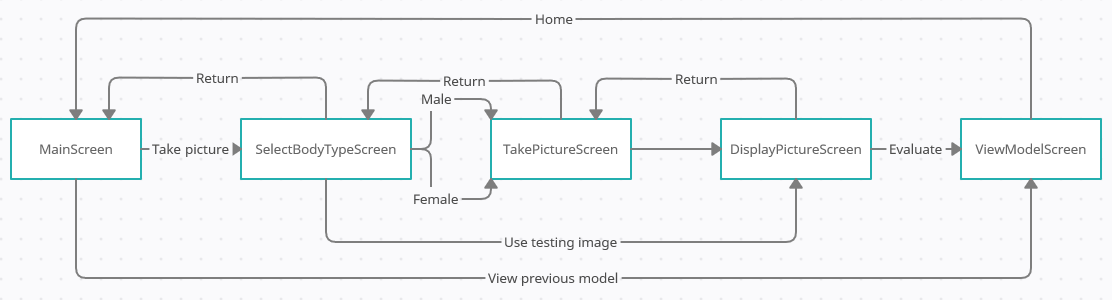
\includegraphics[width=1\textwidth]{appflowchart}
    \caption{Programmablauf der App}
    \label{img:appflowchart}
\end{figure}

In \ref{img:appflowchart} ist der Programmablauf der App dargestellt. Die einzelnen Screens und deren Funktionen werden in den folgenden Abschnitten erläutert. \newline
Da das Design kein Hauptmerkmal der Anwendung ist, wurde eine simple Benutzeroberfläche erstellt. Diese beruht auf einem Dark-Design und setzt Akzente in Blau.

\pagebreak
\section{MainScreen}
\label{sec:mainscreen}
\begin{figure}[htpb]
    \centering
    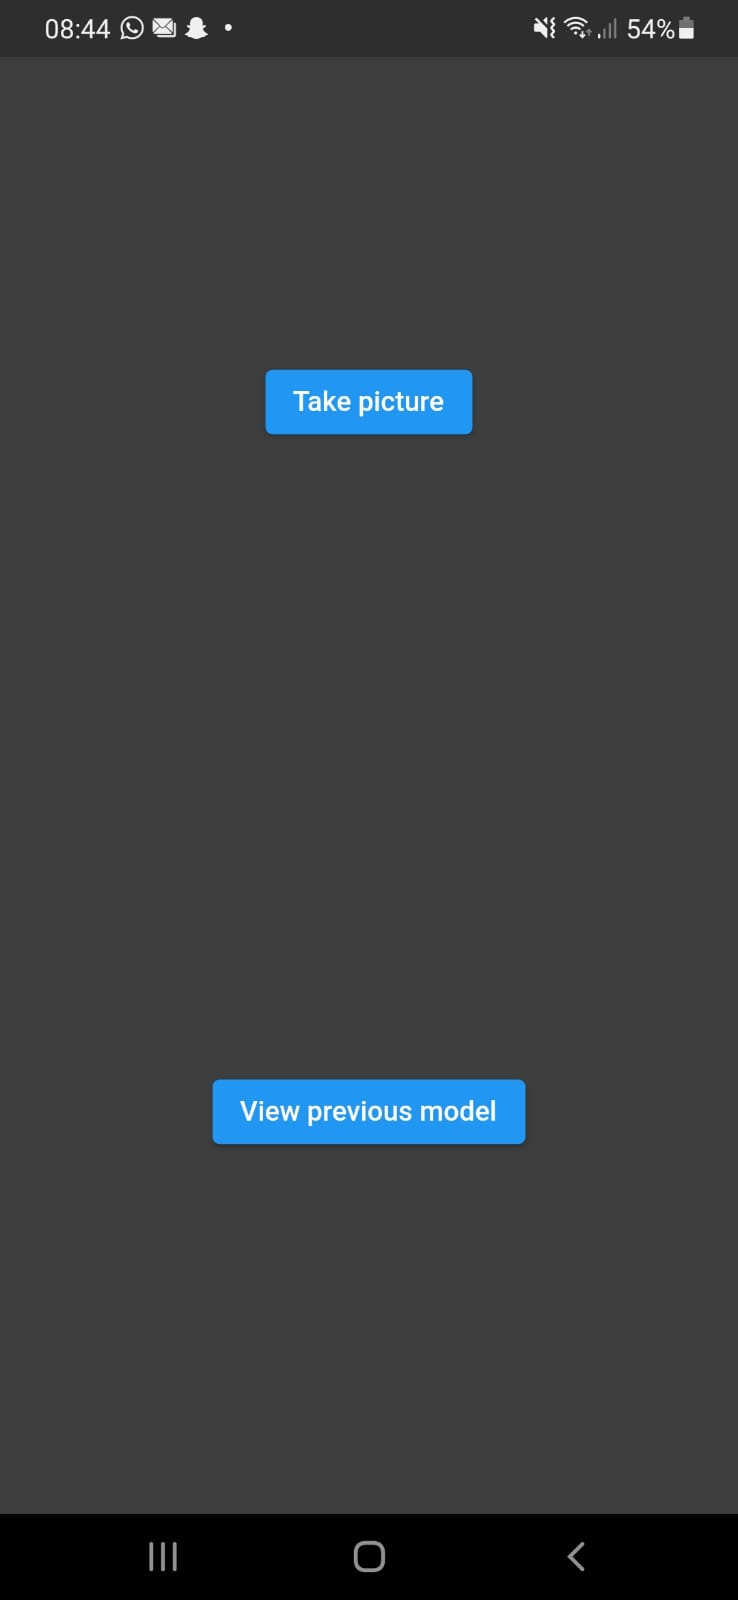
\includegraphics[width=0.3\textwidth]{mainscreen}
    \caption{Der Mainscreen der App}
    \label{img:mainscreen}
\end{figure}

\begin{figure}[htpb]
    \centering
    
\includegraphics[width=0.7\textwidth]{nomodel}
    \caption{Error-Message}
    \label{img:nomodel}
\end{figure}

Der Startbildschirm der Anwendung (\ref{img:mainscreen}) verfügt über zwei Buttons: \glqq{}Take picture\grqq{} und \glqq{}View previous model\grqq{}. \newline
Mit \glqq{}View previous model\grqq{} wird der ViewModelScreen (\ref{img:viewmodel}) aufgerufen und das zuletzt generierte 3D-Modell angezeigt. Befindet sich auf dem Gerät 
kein zuvor generiertes Modell, so wird ein Popup mit einer Error-Message angezeigt (\ref{img:nomodel}). Diese weißt darauf hin, dass kein Modell vorhanden ist und dieses somit zuerst 
durch Aufnehmen und Auswerten eines Fotos generiert werden muss.

Sobald der Startbildschirm generiert wird, werden die auf dem Smartphone verfügbaren Kameras gescannt und in einer Liste gespeichert. Aus dieser Liste wird die Rückkamera 
ausgelsesen und gespeichert. Die Kamera wird später in \ref{sec:takepicture} benötigt. Das Auslesen und Auswerten der Gerätekameras kann etwas Zeit in Anspruch nehmen, weshalb dies 
bereits im Mainscreen passiert und nicht erst beim Aufrufen von TakePictureScreen.

Wird der Button \glqq{}Take picture\grqq{} gedrückt, so wird der SelectBodyTypeScreen generiert und diesem die zuvor gespeicherte Kamera übergeben.

\clearpage
\section{SelectBodyTypeScreen}
\begin{figure}[htpb]
    \centering
    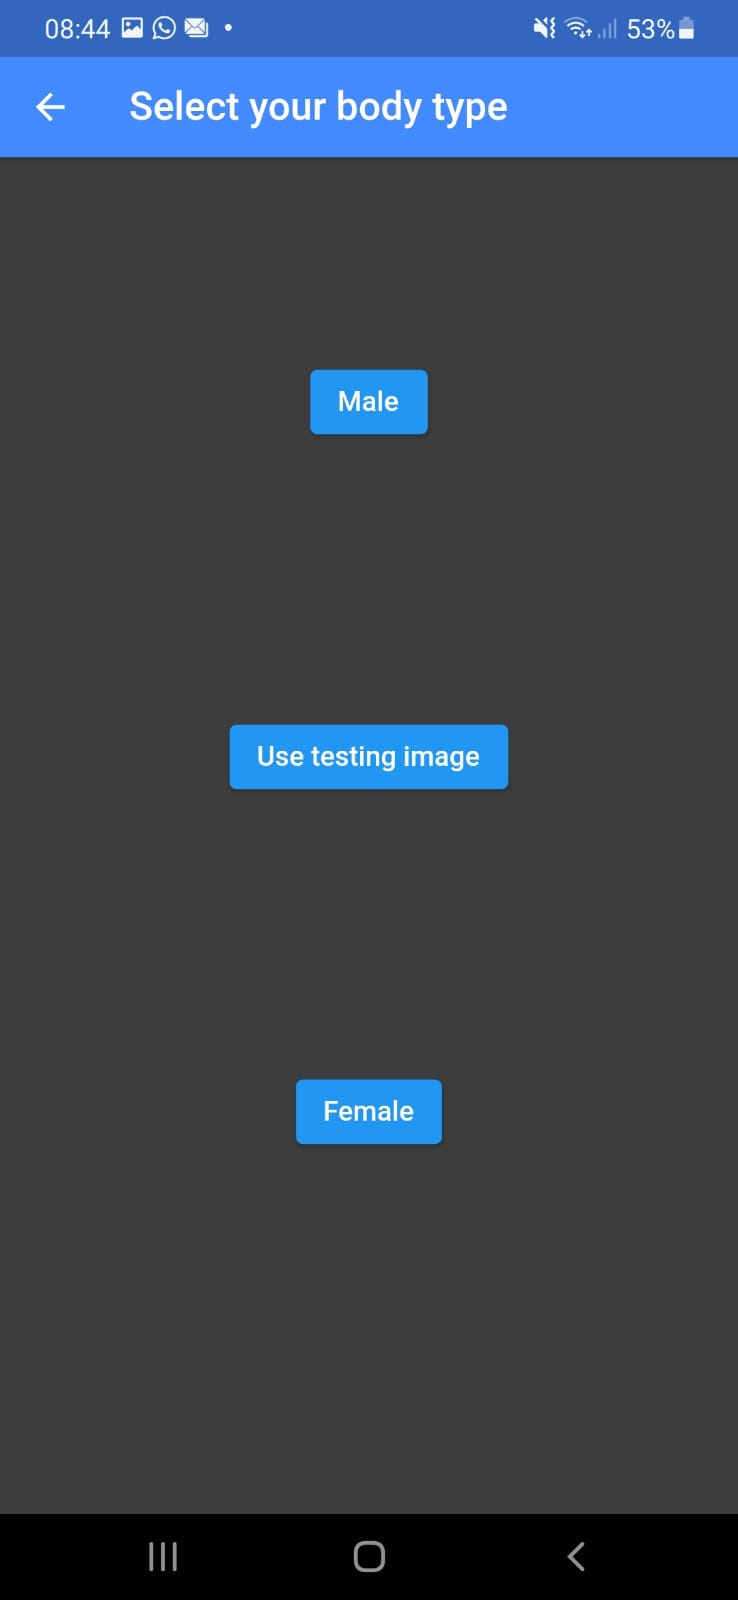
\includegraphics[width=0.3\textwidth]{selectbodytype}
    \caption{Auswahl des Körpertyps}
    \label{img:selectbodytype}
\end{figure}

Auf dem SelectBodyTypeScreen sind drei Buttons vorhanden: \glqq{}Male\grqq{}, \glqq{}Use testing image\grqq{} und \glqq{}Female\grqq{}. Zusätzlich ist eine Statusleiste vorhanden, 
welche zurück zum vorherigen Screen leitet.

Der Button \glqq{}Use testing image\grqq{} leitet den Nutzer direkt zum DisplayPictureScreen (\ref{sec:displaypicture}). Dort wird ein Beispielbild eines Entwicklers in der ZOZOSUIT 
angezeigt, welches anschließend ausgewertet werden kann. \newline
Diese Funktion ist sinnvoll, wenn man die Anwendung testen will und keinen eigenen ZOZOSUIT besitzt oder wenn man den Prozess des An- und Ausziehens des ZOZOSUIT umgehen will.

Die Buttons \glqq{}Male\grqq{} und \glqq{}Female\grqq{} leiten den Nutzer zum TakePictureScreen weiter. Hierbei wird die Variable \textit{gender} übergeben, welche bei der Generierung 
des 3D-Modells benötigt wird. Das drücken eines Buttons setzt dabei die Variable auf das dem Button entsprechende Geschlecht.

\clearpage
\section{TakePictureScreen}
\label{sec:takepicture}
\begin{figure}[htpb]
    \centering
    
\includegraphics[width=0.3\textwidth]{takepicture}
    \caption{Aufnehmen eines Bildes}
    \label{img:takepicture}
\end{figure}

Der TakePictureScreen verfügt über einen Button mit einem Kamerasymbol und eine Statusleiste, welche den Nutzer zum vorherigen Screen leitet.

In der Mitte des Bildschirms wird der aktuelle Kamerafeed der Rückkamera angezeigt, welche bereits in \ref{sec:mainscreen} bereitgestellt wurde. Wird der Kamerabutton gedrückt, 
so wird ein Bild aufgenommen und temporär gespeichert. Der Pfad zum aktuellen Bild und das vom SelectBodyTypeScreen erhaltene Geschlecht werden an den DisplayPictureScreen weitergeleitet, 
welcher nun generiert wird.

\clearpage
\section{DisplayPictureScreen}
\label{sec:displaypicture}
\begin{figure}[htpb]
    \centering
    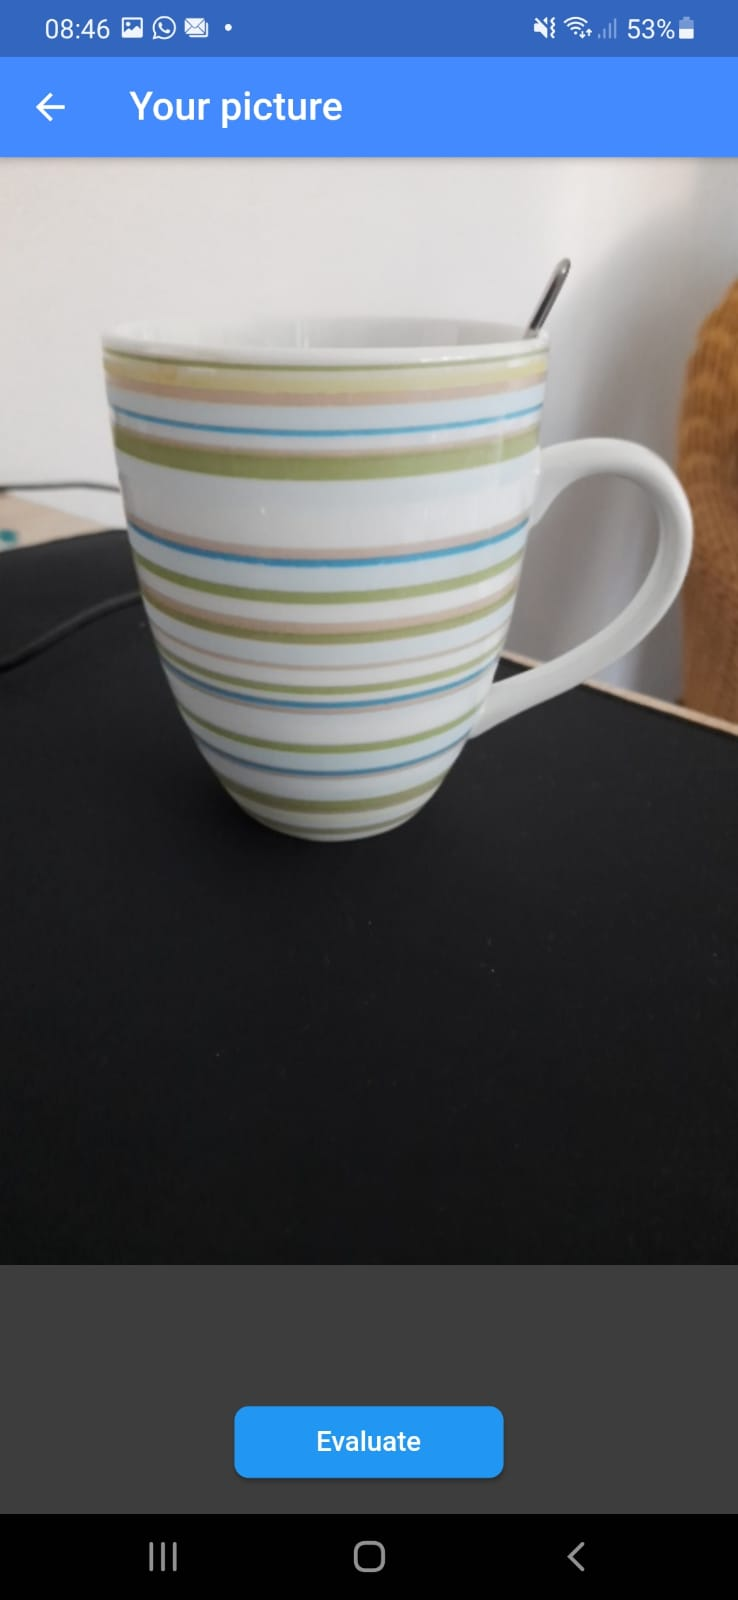
\includegraphics[width=0.3\textwidth]{displaypicture}
    \caption{Anzeigen des aufgenommenen Bildes}
    \label{img:displaypicture}
\end{figure}

Der DisplayPictureScreen zeigt das zuvor aufgenommene Bild an und besitzt den Button \glqq{}Evaluate\grqq{} und eine Statusleiste, welche den Nutzer zum vorherigen Screen leitet. \newline
Wurde im SelectBodyTypeScreen der Button \glqq{}Use test image\grqq{} gedrückt, so wird eine Variante dieses Screens angezeigt. Der einzige Unterschied liegt dabei darin, dass nicht 
das zuvor aufgenommene Bild, sondern ein aus den, in der App enthaltenen, Assets geladenes Bild, angezeigt wird.

Wird der Button gedrückt, so zeigt dieser eine Ladeanimation an, bis alle durch den Button aufgerufenen Funktionen abgeschlossen sind.

Zuerst wird das aktuelle Bild zu einem Base64-String (\cite{misc:base64}) konvertiert. Der somit generierte String wird nun mit dem erhaltenen Geschlecht per POST-Request an den Server 
gesendet. Der Server wertet die Daten aus und generiert daraus ein 3D-Modell als .glb-Datei. Diese Datei wird zu Base64 kodiert und an die App zurückgesendet. \newline
Der Base64-String wird nun dekodiert und in dem appspezifischen Speicher gespeichert. Hierbei muss darauf geachtet werden, dass die Speicherorte auf Android und iOS Geräten 
verschieden sind. Deshalb wird das Betriebssystem des Smartphones bestimmt und daraus lässt sich der Pfad zum Speicherort für appspezifische Dateien generieren. Die dekodierte Datei 
wird nun an dem erhaltenen Pfad gespeichert. \newline
Der Pfad zum gespeicherten 3D-Modell (die .glb Datei) wird gespeichert und an den ViewModelScreen weitergegeben, welcher nun generiert wird.

\clearpage
\section{ViewModelScreen}
\begin{figure}[htpb]
    \centering
    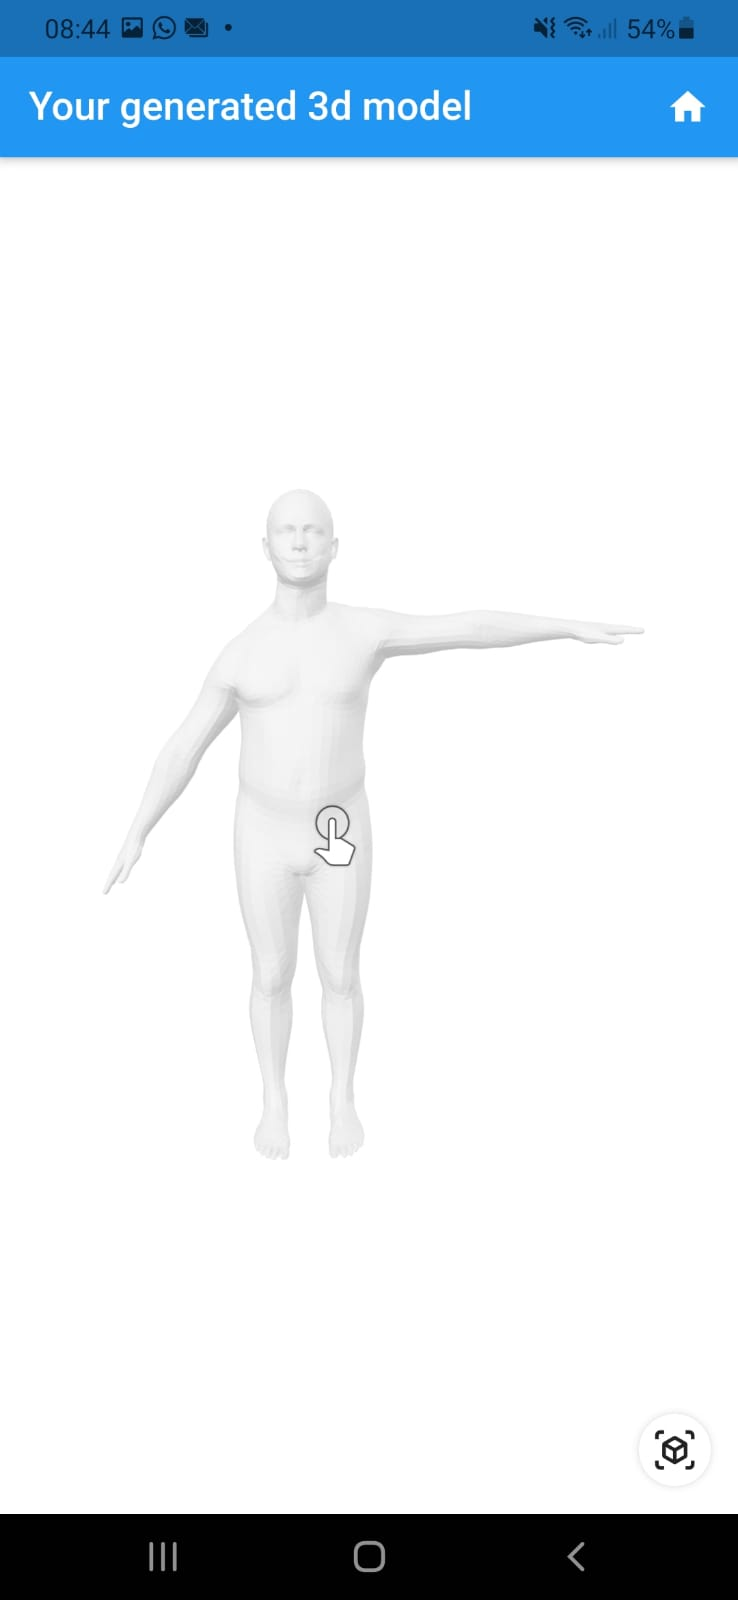
\includegraphics[width=0.3\textwidth]{viewmodel}
    \caption{Anzeigen des 3D-Modells}
    \label{img:viewmodel}
\end{figure}

Der ViewModelScreen erhält einen Pfad zu einer .glb-Datei. Diese Datei wird gerendert und als drehbares 3D-Modell gerendert. Zusätzlich ist eine Statusleiste mit einem Home-Button 
vorhanden, welcher den Nutzer zurück zum MainScreen bringt. 

Um das 3D-Modell zu rendern verwendet die App das Plugin \textit{Model Viewer} (\cite{misc:modelviewer}). \textit{Model Viewer} erstellt eine WebView und startet somit einen Server 
innerhalb der App. Das 3D-Modell wird in einem Browser mithilfe von WebGL gerendert und in der App dargestellt.

Der Button rechts unten lädt das Modell im von Google erstellten model-viewer, auf welchem dieses Plugin basiert.

\pagebreak
\section{Probleme}


\chapter{App}
\label{ch:app}

Da die App Kamerafunktionen verwendet, wird auf dem Smartphone ein \acrshort{api}-Level von 21 vorausgesetz. Dies entspricht Android 5.0, welches 2014 erschienen ist.

\section{Aufbau}
\begin{figure}[htpb]
    \centering
    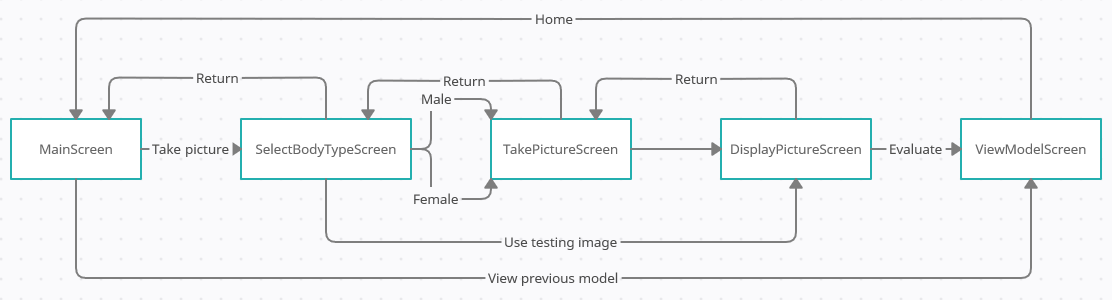
\includegraphics[width=1\textwidth]{appflowchart}
    \caption{Programmablauf der App}
    \label{img:appflowchart}
\end{figure}

In \ref{img:appflowchart} ist der Programmablauf der App dargestellt. Die einzelnen Screens und deren Funktionen werden in den folgenden Abschnitten erläutert. \newline
Da das Design kein Hauptmerkmal der Anwendung ist, wurde eine simple Benutzeroberfläche erstellt. Diese beruht auf einem Dark-Design und setzt Akzente in Blau.

\pagebreak
\section{MainScreen}
\label{sec:mainscreen}
\begin{figure}[htpb]
    \centering
    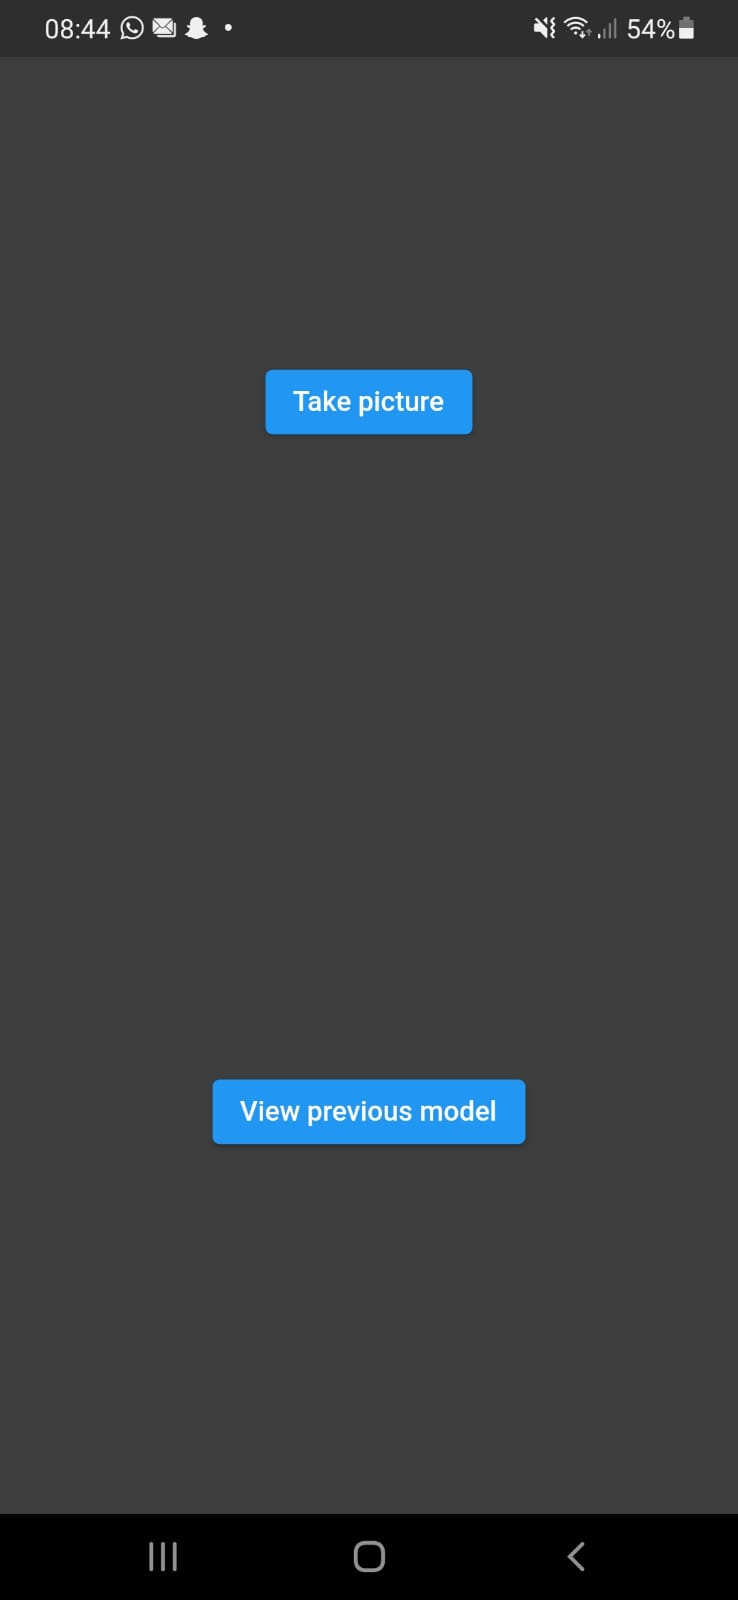
\includegraphics[width=0.3\textwidth]{mainscreen}
    \caption{Der Mainscreen der App}
    \label{img:mainscreen}
\end{figure}

\begin{figure}[htpb]
    \centering
    
\includegraphics[width=0.7\textwidth]{nomodel}
    \caption{Error-Message}
    \label{img:nomodel}
\end{figure}

Der Startbildschirm der Anwendung (\ref{img:mainscreen}) verfügt über zwei Buttons: \glqq{}Take picture\grqq{} und \glqq{}View previous model\grqq{}. \newline
Mit \glqq{}View previous model\grqq{} wird der ViewModelScreen (\ref{img:viewmodel}) aufgerufen und das zuletzt generierte 3D-Modell angezeigt. Befindet sich auf dem Gerät 
kein zuvor generiertes Modell, so wird ein Popup mit einer Error-Message angezeigt (\ref{img:nomodel}). Diese weißt darauf hin, dass kein Modell vorhanden ist und dieses somit zuerst 
durch Aufnehmen und Auswerten eines Fotos generiert werden muss.

Sobald der Startbildschirm generiert wird, werden die auf dem Smartphone verfügbaren Kameras gescannt und in einer Liste gespeichert. Aus dieser Liste wird die Rückkamera 
ausgelsesen und gespeichert. Die Kamera wird später in \ref{sec:takepicture} benötigt. Das Auslesen und Auswerten der Gerätekameras kann etwas Zeit in Anspruch nehmen, weshalb dies 
bereits im Mainscreen passiert und nicht erst beim Aufrufen von TakePictureScreen.

Wird der Button \glqq{}Take picture\grqq{} gedrückt, so wird der SelectBodyTypeScreen generiert und diesem die zuvor gespeicherte Kamera übergeben.

\clearpage
\section{SelectBodyTypeScreen}
\begin{figure}[htpb]
    \centering
    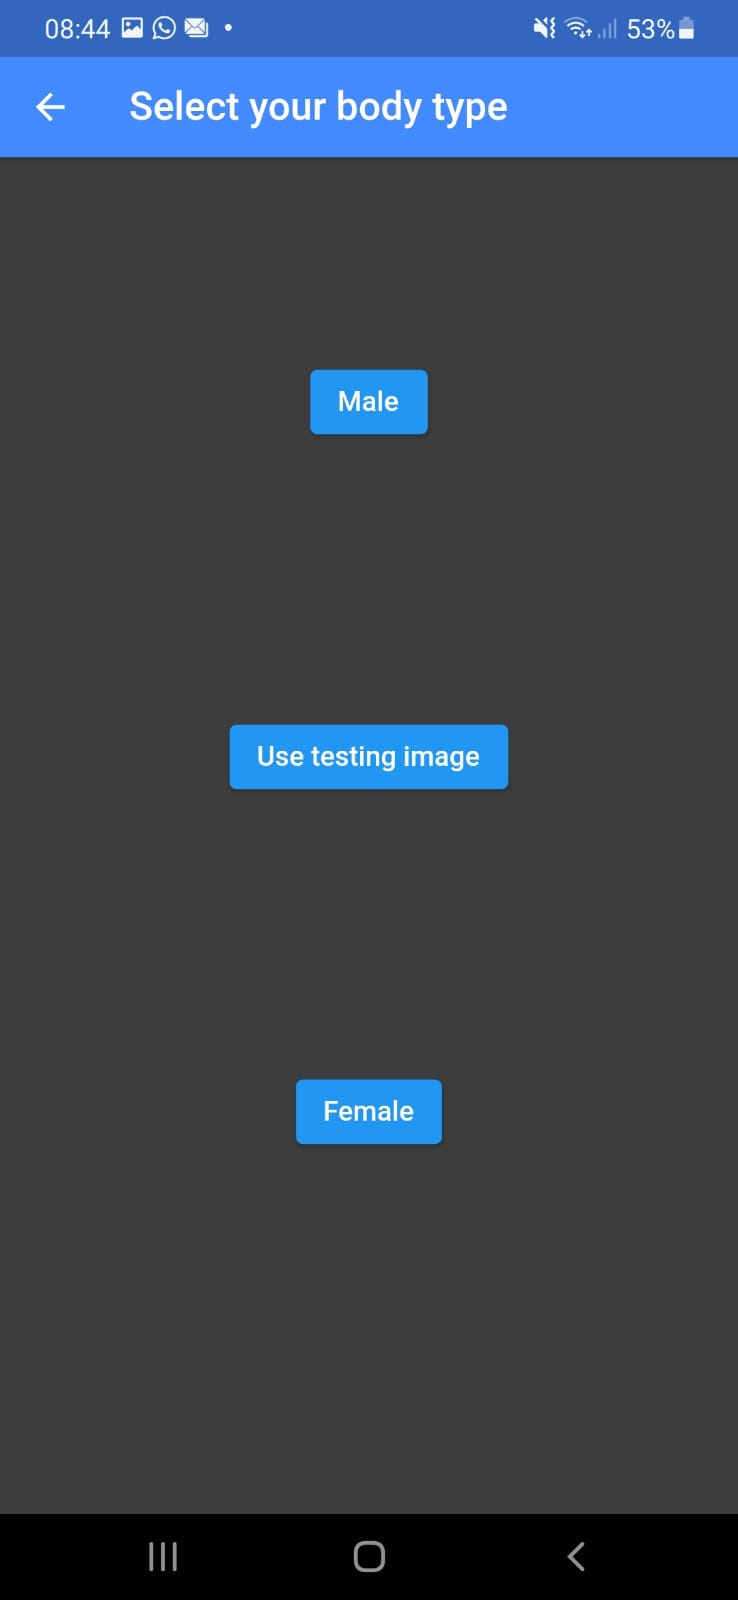
\includegraphics[width=0.3\textwidth]{selectbodytype}
    \caption{Auswahl des Körpertyps}
    \label{img:selectbodytype}
\end{figure}

Auf dem SelectBodyTypeScreen sind drei Buttons vorhanden: \glqq{}Male\grqq{}, \glqq{}Use testing image\grqq{} und \glqq{}Female\grqq{}. Zusätzlich ist eine Statusleiste vorhanden, 
welche zurück zum vorherigen Screen leitet.

Der Button \glqq{}Use testing image\grqq{} leitet den Nutzer direkt zum DisplayPictureScreen (\ref{sec:displaypicture}). Dort wird ein Beispielbild eines Entwicklers in der ZOZOSUIT 
angezeigt, welches anschließend ausgewertet werden kann. \newline
Diese Funktion ist sinnvoll, wenn man die Anwendung testen will und keinen eigenen ZOZOSUIT besitzt oder wenn man den Prozess des An- und Ausziehens des ZOZOSUIT umgehen will.

Die Buttons \glqq{}Male\grqq{} und \glqq{}Female\grqq{} leiten den Nutzer zum TakePictureScreen weiter. Hierbei wird die Variable \textit{gender} übergeben, welche bei der Generierung 
des 3D-Modells benötigt wird. Das drücken eines Buttons setzt dabei die Variable auf das dem Button entsprechende Geschlecht.

\clearpage
\section{TakePictureScreen}
\label{sec:takepicture}
\begin{figure}[htpb]
    \centering
    
\includegraphics[width=0.3\textwidth]{takepicture}
    \caption{Aufnehmen eines Bildes}
    \label{img:takepicture}
\end{figure}

Der TakePictureScreen verfügt über einen Button mit einem Kamerasymbol und eine Statusleiste, welche den Nutzer zum vorherigen Screen leitet.

In der Mitte des Bildschirms wird der aktuelle Kamerafeed der Rückkamera angezeigt, welche bereits in \ref{sec:mainscreen} bereitgestellt wurde. Wird der Kamerabutton gedrückt, 
so wird ein Bild aufgenommen und temporär gespeichert. Der Pfad zum aktuellen Bild und das vom SelectBodyTypeScreen erhaltene Geschlecht werden an den DisplayPictureScreen weitergeleitet, 
welcher nun generiert wird.

\clearpage
\section{DisplayPictureScreen}
\label{sec:displaypicture}
\begin{figure}[htpb]
    \centering
    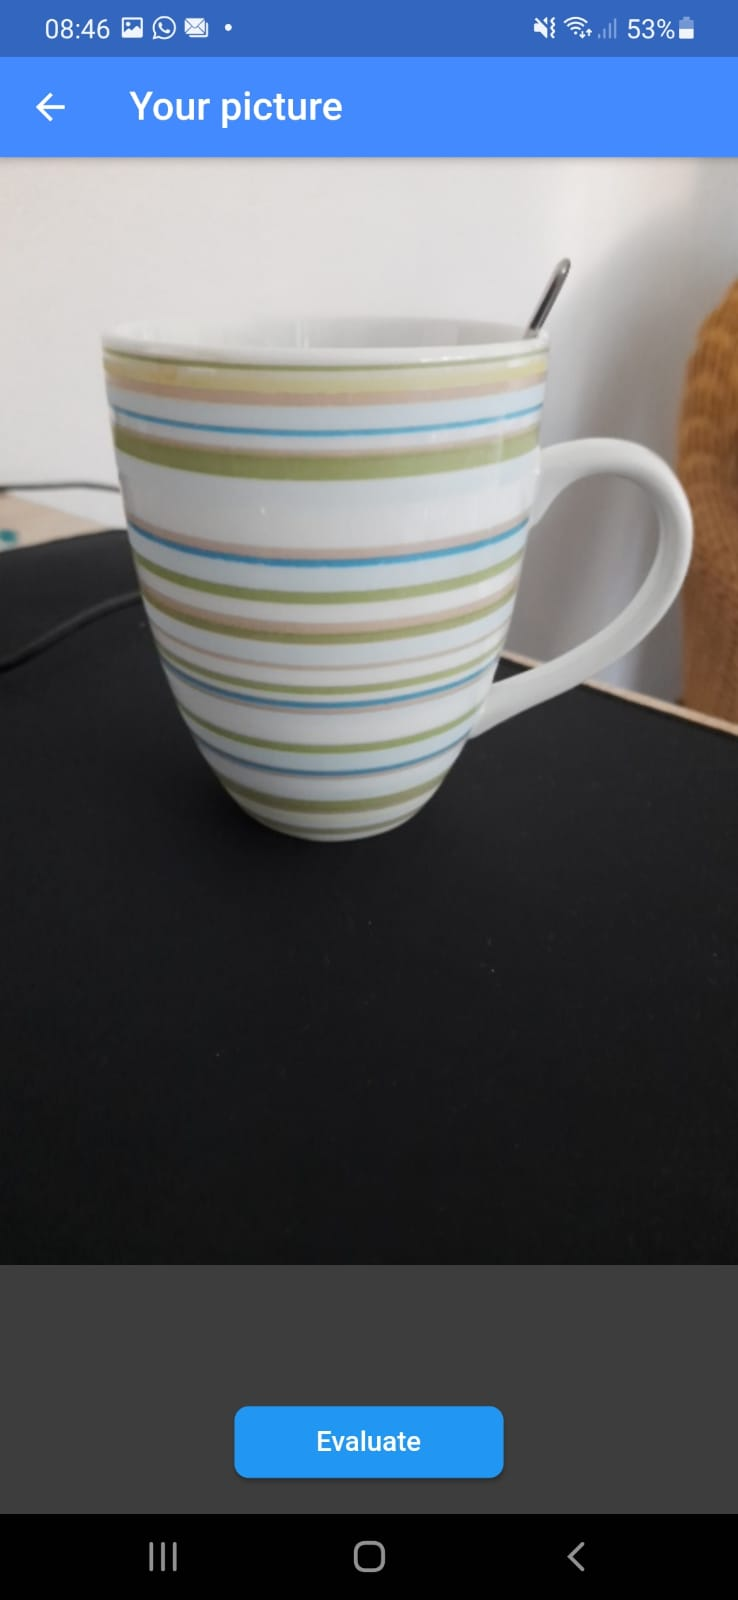
\includegraphics[width=0.3\textwidth]{displaypicture}
    \caption{Anzeigen des aufgenommenen Bildes}
    \label{img:displaypicture}
\end{figure}

Der DisplayPictureScreen zeigt das zuvor aufgenommene Bild an und besitzt den Button \glqq{}Evaluate\grqq{} und eine Statusleiste, welche den Nutzer zum vorherigen Screen leitet. \newline
Wurde im SelectBodyTypeScreen der Button \glqq{}Use test image\grqq{} gedrückt, so wird eine Variante dieses Screens angezeigt. Der einzige Unterschied liegt dabei darin, dass nicht 
das zuvor aufgenommene Bild, sondern ein aus den, in der App enthaltenen, Assets geladenes Bild, angezeigt wird.

Wird der Button gedrückt, so zeigt dieser eine Ladeanimation an, bis alle durch den Button aufgerufenen Funktionen abgeschlossen sind.

Zuerst wird das aktuelle Bild zu einem Base64-String (\cite{misc:base64}) konvertiert. Der somit generierte String wird nun mit dem erhaltenen Geschlecht per POST-Request an den Server 
gesendet. Der Server wertet die Daten aus und generiert daraus ein 3D-Modell als .glb-Datei. Diese Datei wird zu Base64 kodiert und an die App zurückgesendet. \newline
Der Base64-String wird nun dekodiert und in dem appspezifischen Speicher gespeichert. Hierbei muss darauf geachtet werden, dass die Speicherorte auf Android und iOS Geräten 
verschieden sind. Deshalb wird das Betriebssystem des Smartphones bestimmt und daraus lässt sich der Pfad zum Speicherort für appspezifische Dateien generieren. Die dekodierte Datei 
wird nun an dem erhaltenen Pfad gespeichert. \newline
Der Pfad zum gespeicherten 3D-Modell (die .glb Datei) wird gespeichert und an den ViewModelScreen weitergegeben, welcher nun generiert wird.

\clearpage
\section{ViewModelScreen}
\begin{figure}[htpb]
    \centering
    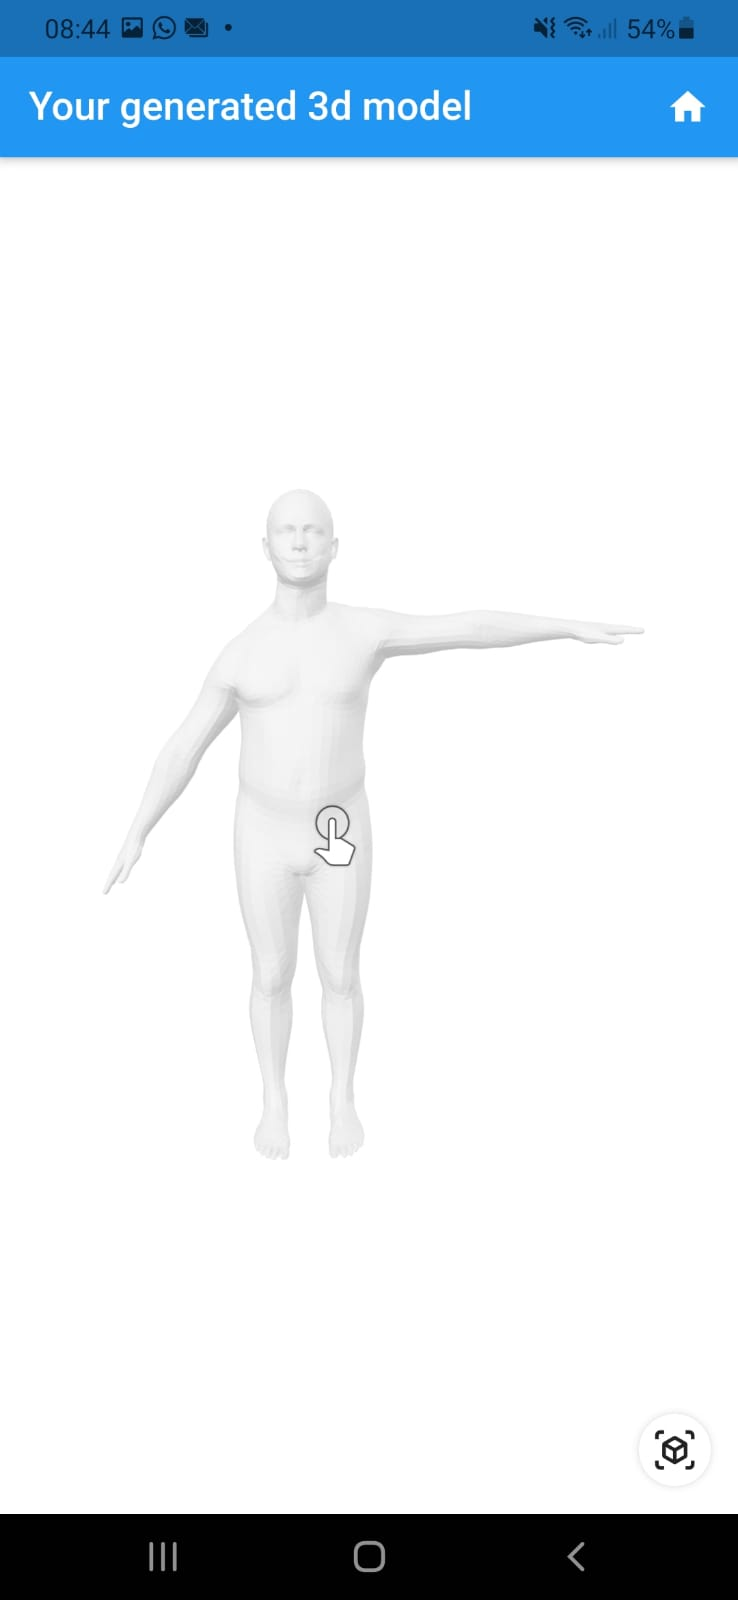
\includegraphics[width=0.3\textwidth]{viewmodel}
    \caption{Anzeigen des 3D-Modells}
    \label{img:viewmodel}
\end{figure}

Der ViewModelScreen erhält einen Pfad zu einer .glb-Datei. Diese Datei wird gerendert und als drehbares 3D-Modell gerendert. Zusätzlich ist eine Statusleiste mit einem Home-Button 
vorhanden, welcher den Nutzer zurück zum MainScreen bringt. 

Um das 3D-Modell zu rendern verwendet die App das Plugin \textit{Model Viewer} (\cite{misc:modelviewer}). \textit{Model Viewer} erstellt eine WebView und startet somit einen Server 
innerhalb der App. Das 3D-Modell wird in einem Browser mithilfe von WebGL gerendert und in der App dargestellt.

Der Button rechts unten lädt das Modell im von Google erstellten model-viewer, auf welchem dieses Plugin basiert.

\pagebreak
\section{Probleme}


\chapter{Zusammenfassung und Ausblick}

klappt zwar mit suit, geht aber theoretisch bessre ohne, zozosuit2 könnte das vermutlich aber schaffen   % Zusammenfassung                

\printbibliography                          % Literaturverzeichnis
\end{document}